\chapter{Systemts grænseflader}

\section{Indledning}
I dette dokument vil der være en beksrivelse af systemets grænseflader. 
Derudover vil der også være beskrivelse af de valg, der er blevet taget i forhold til designet af brugergrænsefladen igennem projektet. 

\section{WebApp}
Der er blevet udarbejdet en række skitser på et tidligt stadie i projektet. Disse skitser er blevet udarbejdet for at give et overblik over funktionaliteten af platformen.


\begin{figure}[ht]
    \centering

\includegraphics[width=0.6\textwidth]{system-interface-pic/Homepage-desktop.pdf}
\caption{Viser forsiden af Converge platformen}
\label{fig:figure2}
\end{figure}

på figur 1.1 viser forsiden af Converge platformen og som er den første side brugeren møder. Her kan brugeren fortage sige forskellige ting såsom: at kunne login, registerer sig, som enten freelancer eller empolyer og derudover kan brugeren læse information om selve platformen og hvordan det er at være en del af den.   
\newpage
\begin{figure}[ht]
    \centering
\includegraphics[width=0.6\textwidth]{system-interface-pic/About.pdf}
\caption{Viser siden hvor brugeren kan læse information om Converge platformen}
\label{fig:figure2}
\end{figure}

Figur 1.2 viser information siden om selve Converge platformen. Her har brugeren muglighed for at læse og blive klogere på platformen.

\begin{figure}[ht]
    \centering
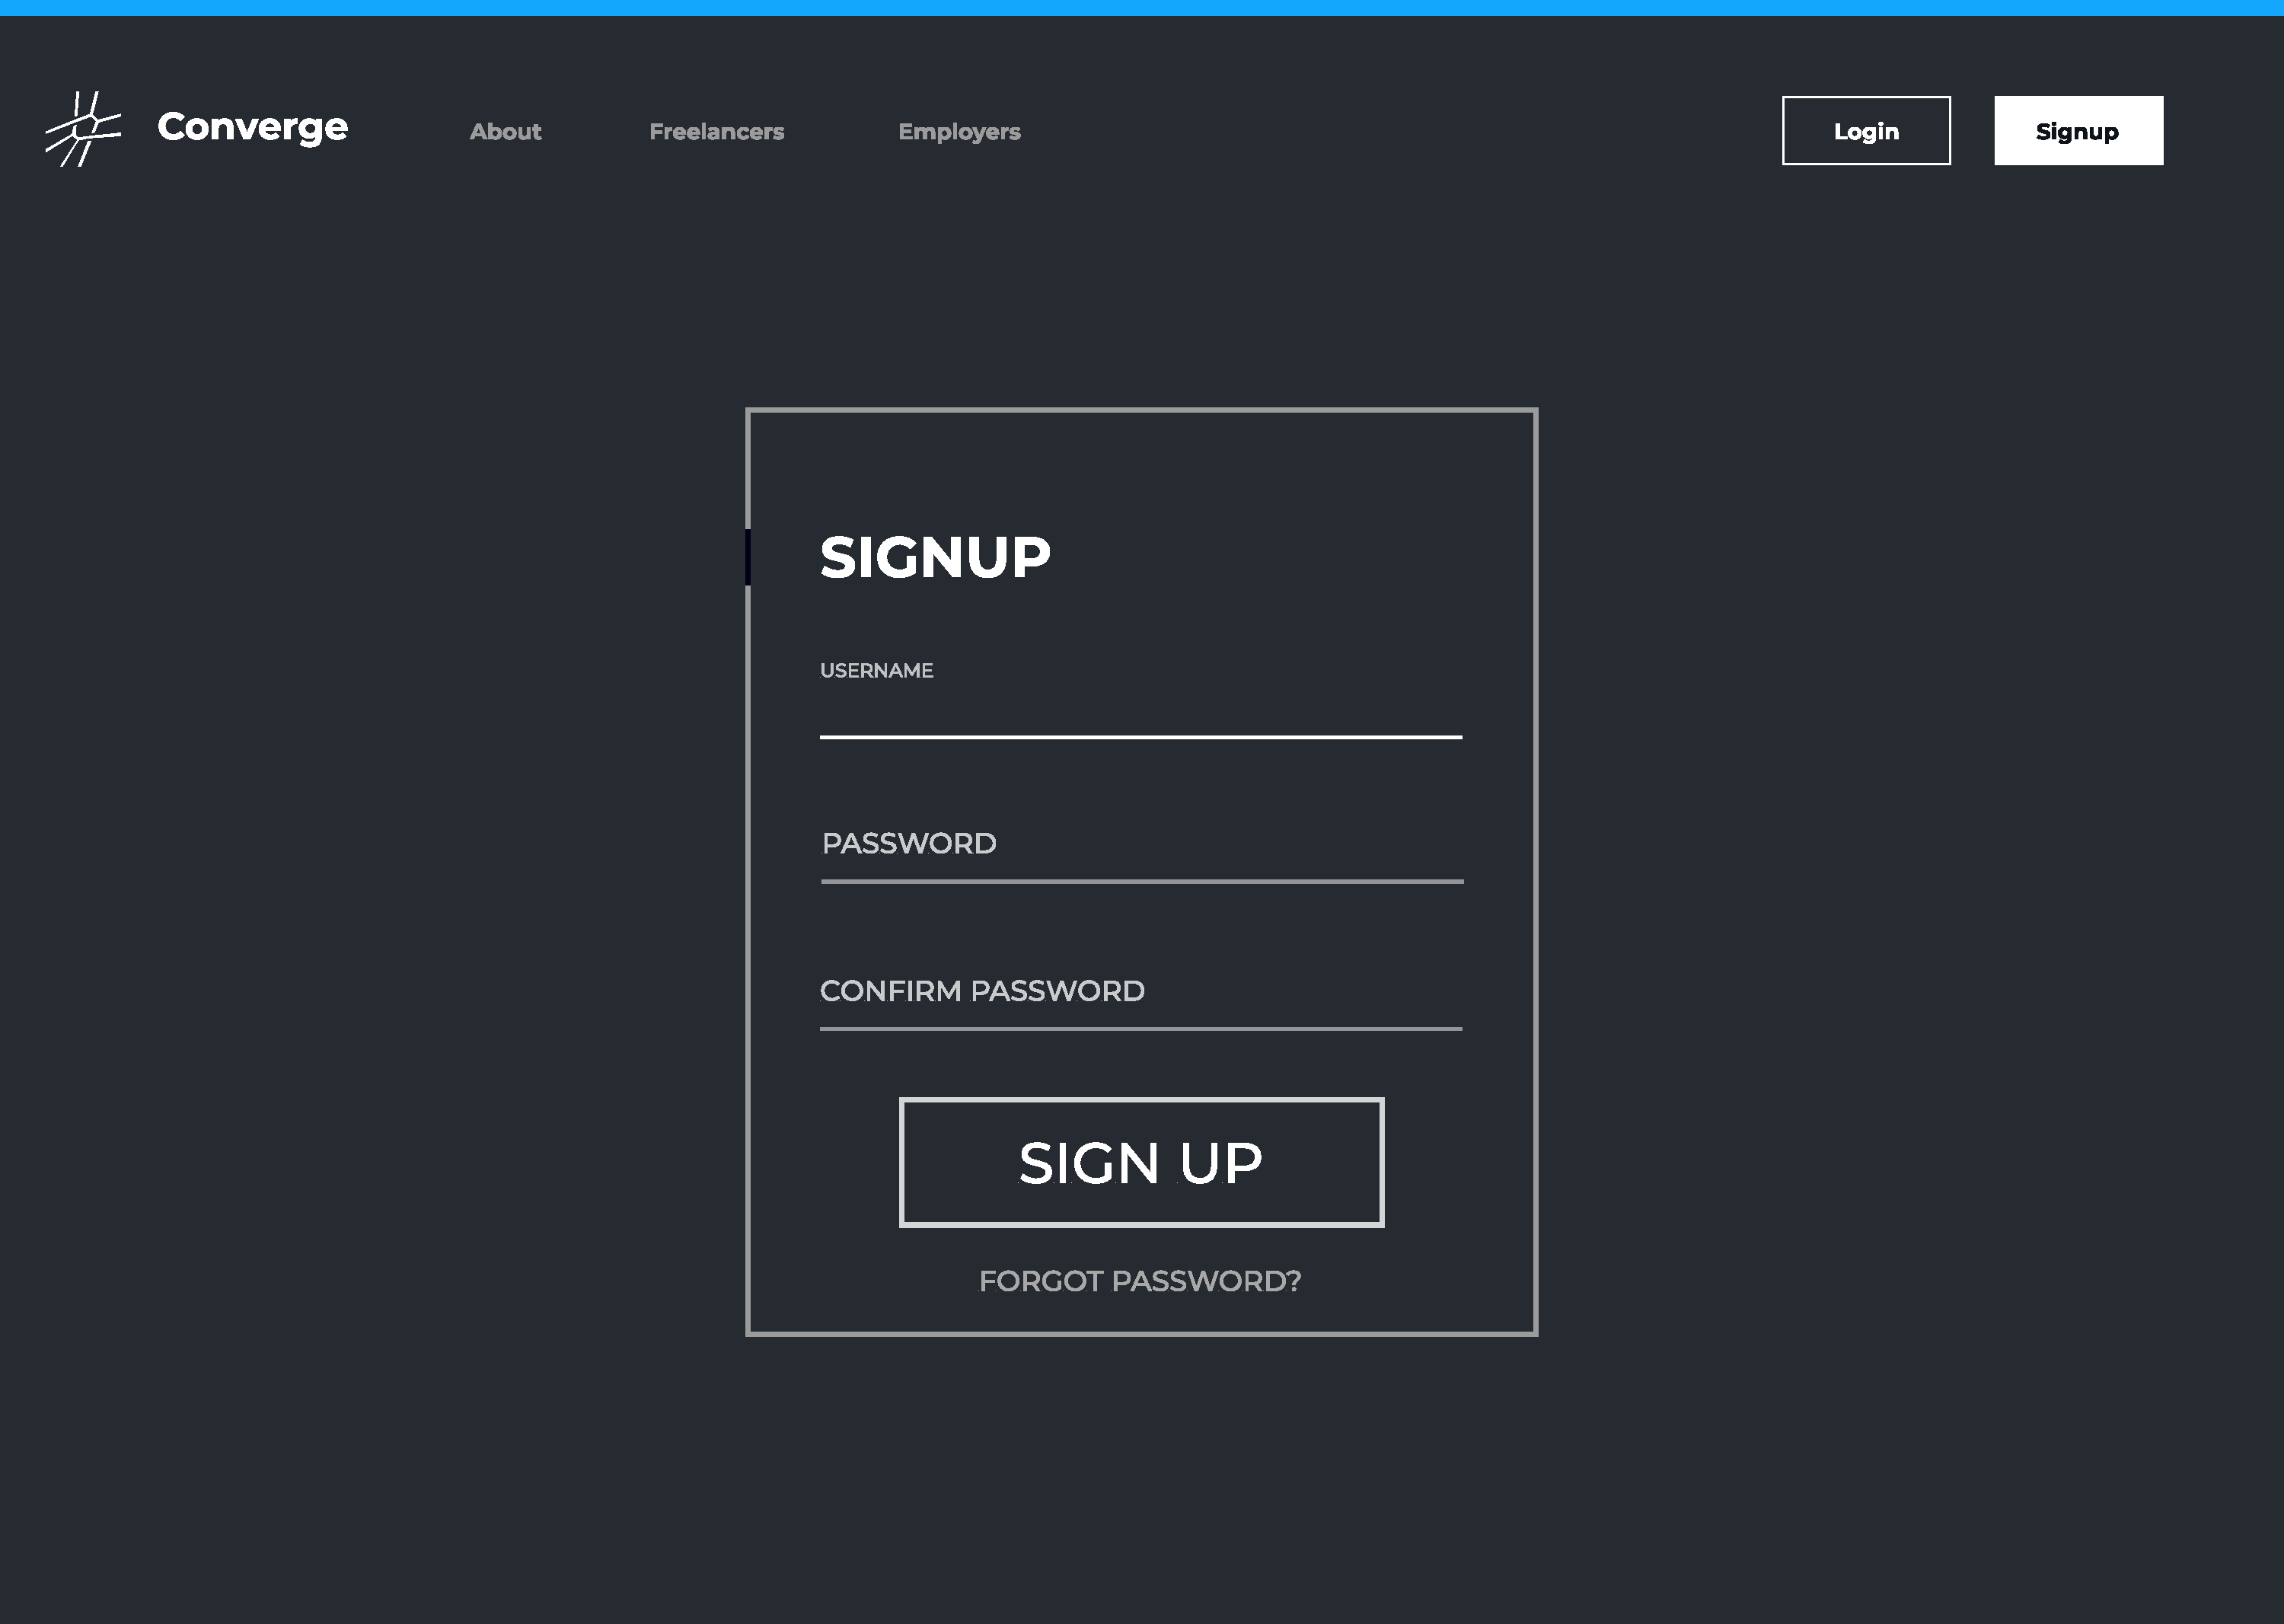
\includegraphics[width=0.6\textwidth]{system-interface-pic/Signup.pdf}
\caption{Viser registerings side}
\label{fig:figure2}
\end{figure}

på figur 1.4 ses registerings siden, hvor brugeren kan registerer sig som bruger på Converge platformen.



\newpage
\begin{figure}[ht]
    \centering
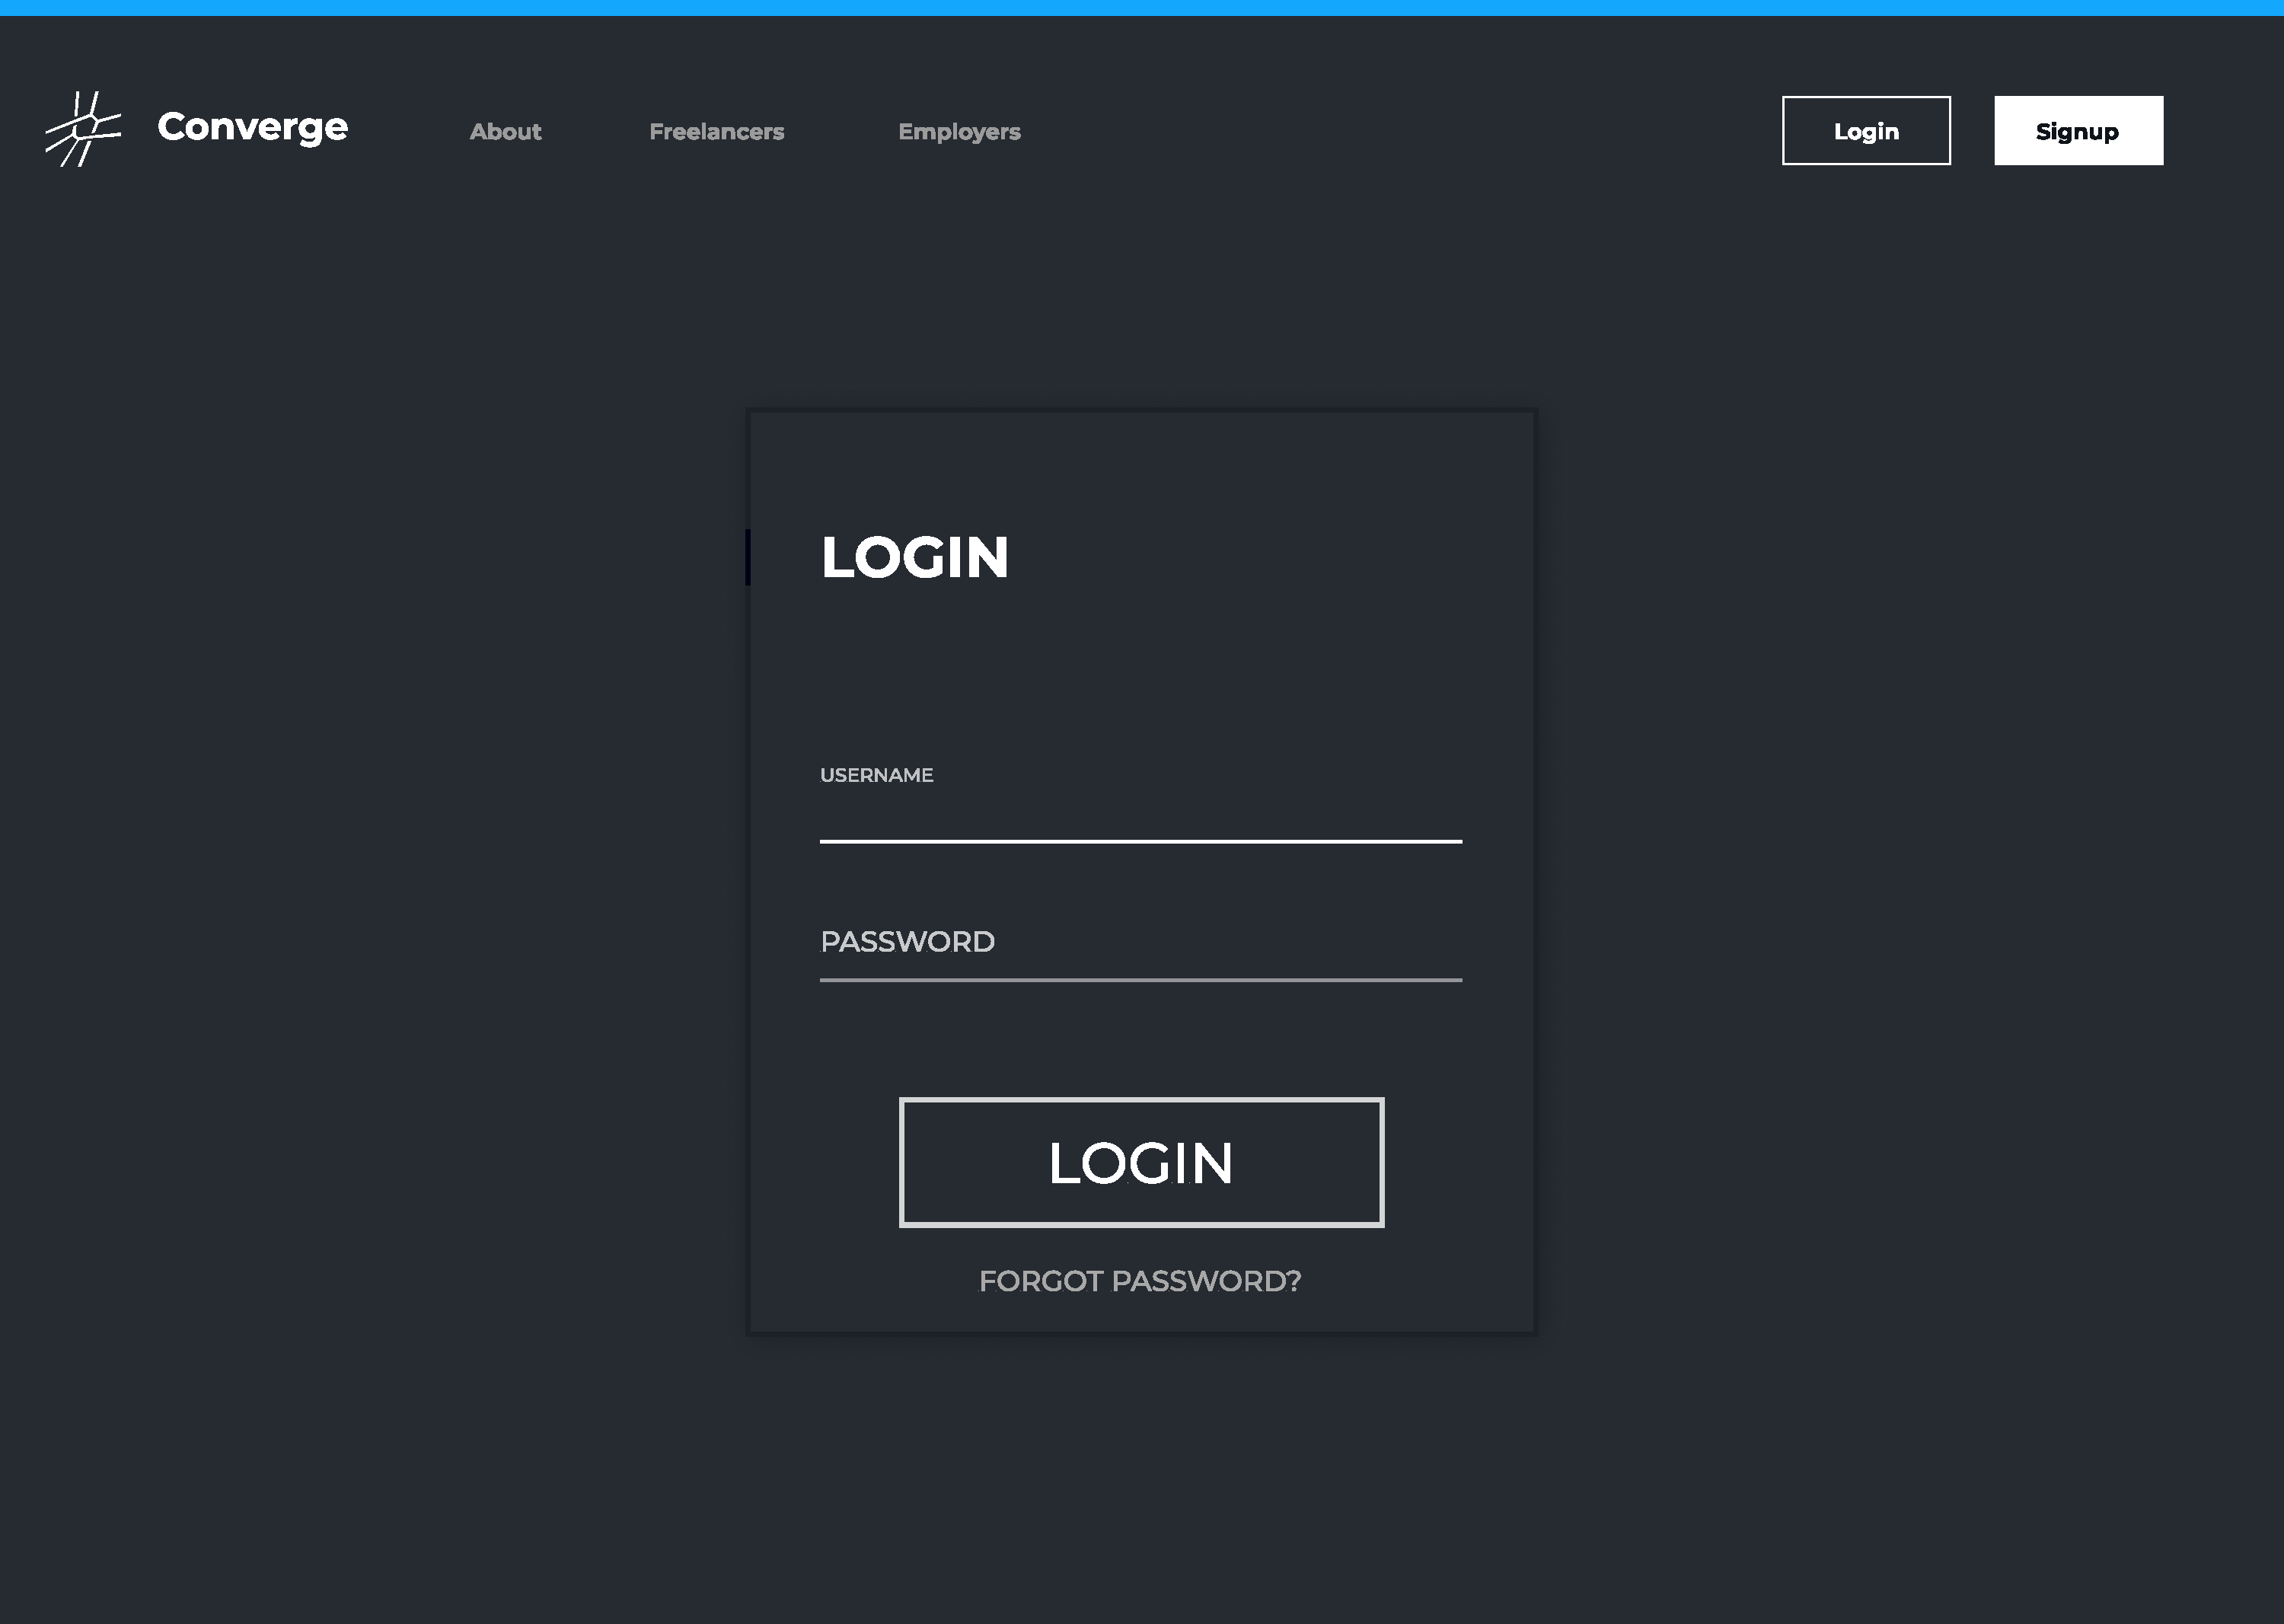
\includegraphics[width=0.6\textwidth]{system-interface-pic/Login.pdf}
\caption{Viser login siden}
\label{fig:figure2}
\end{figure}

På ovenstående figur ses login siden og her har brugeren muglighed for at kunne login med et valid login, som er email og password. 

\begin{figure}[ht]
    \centering
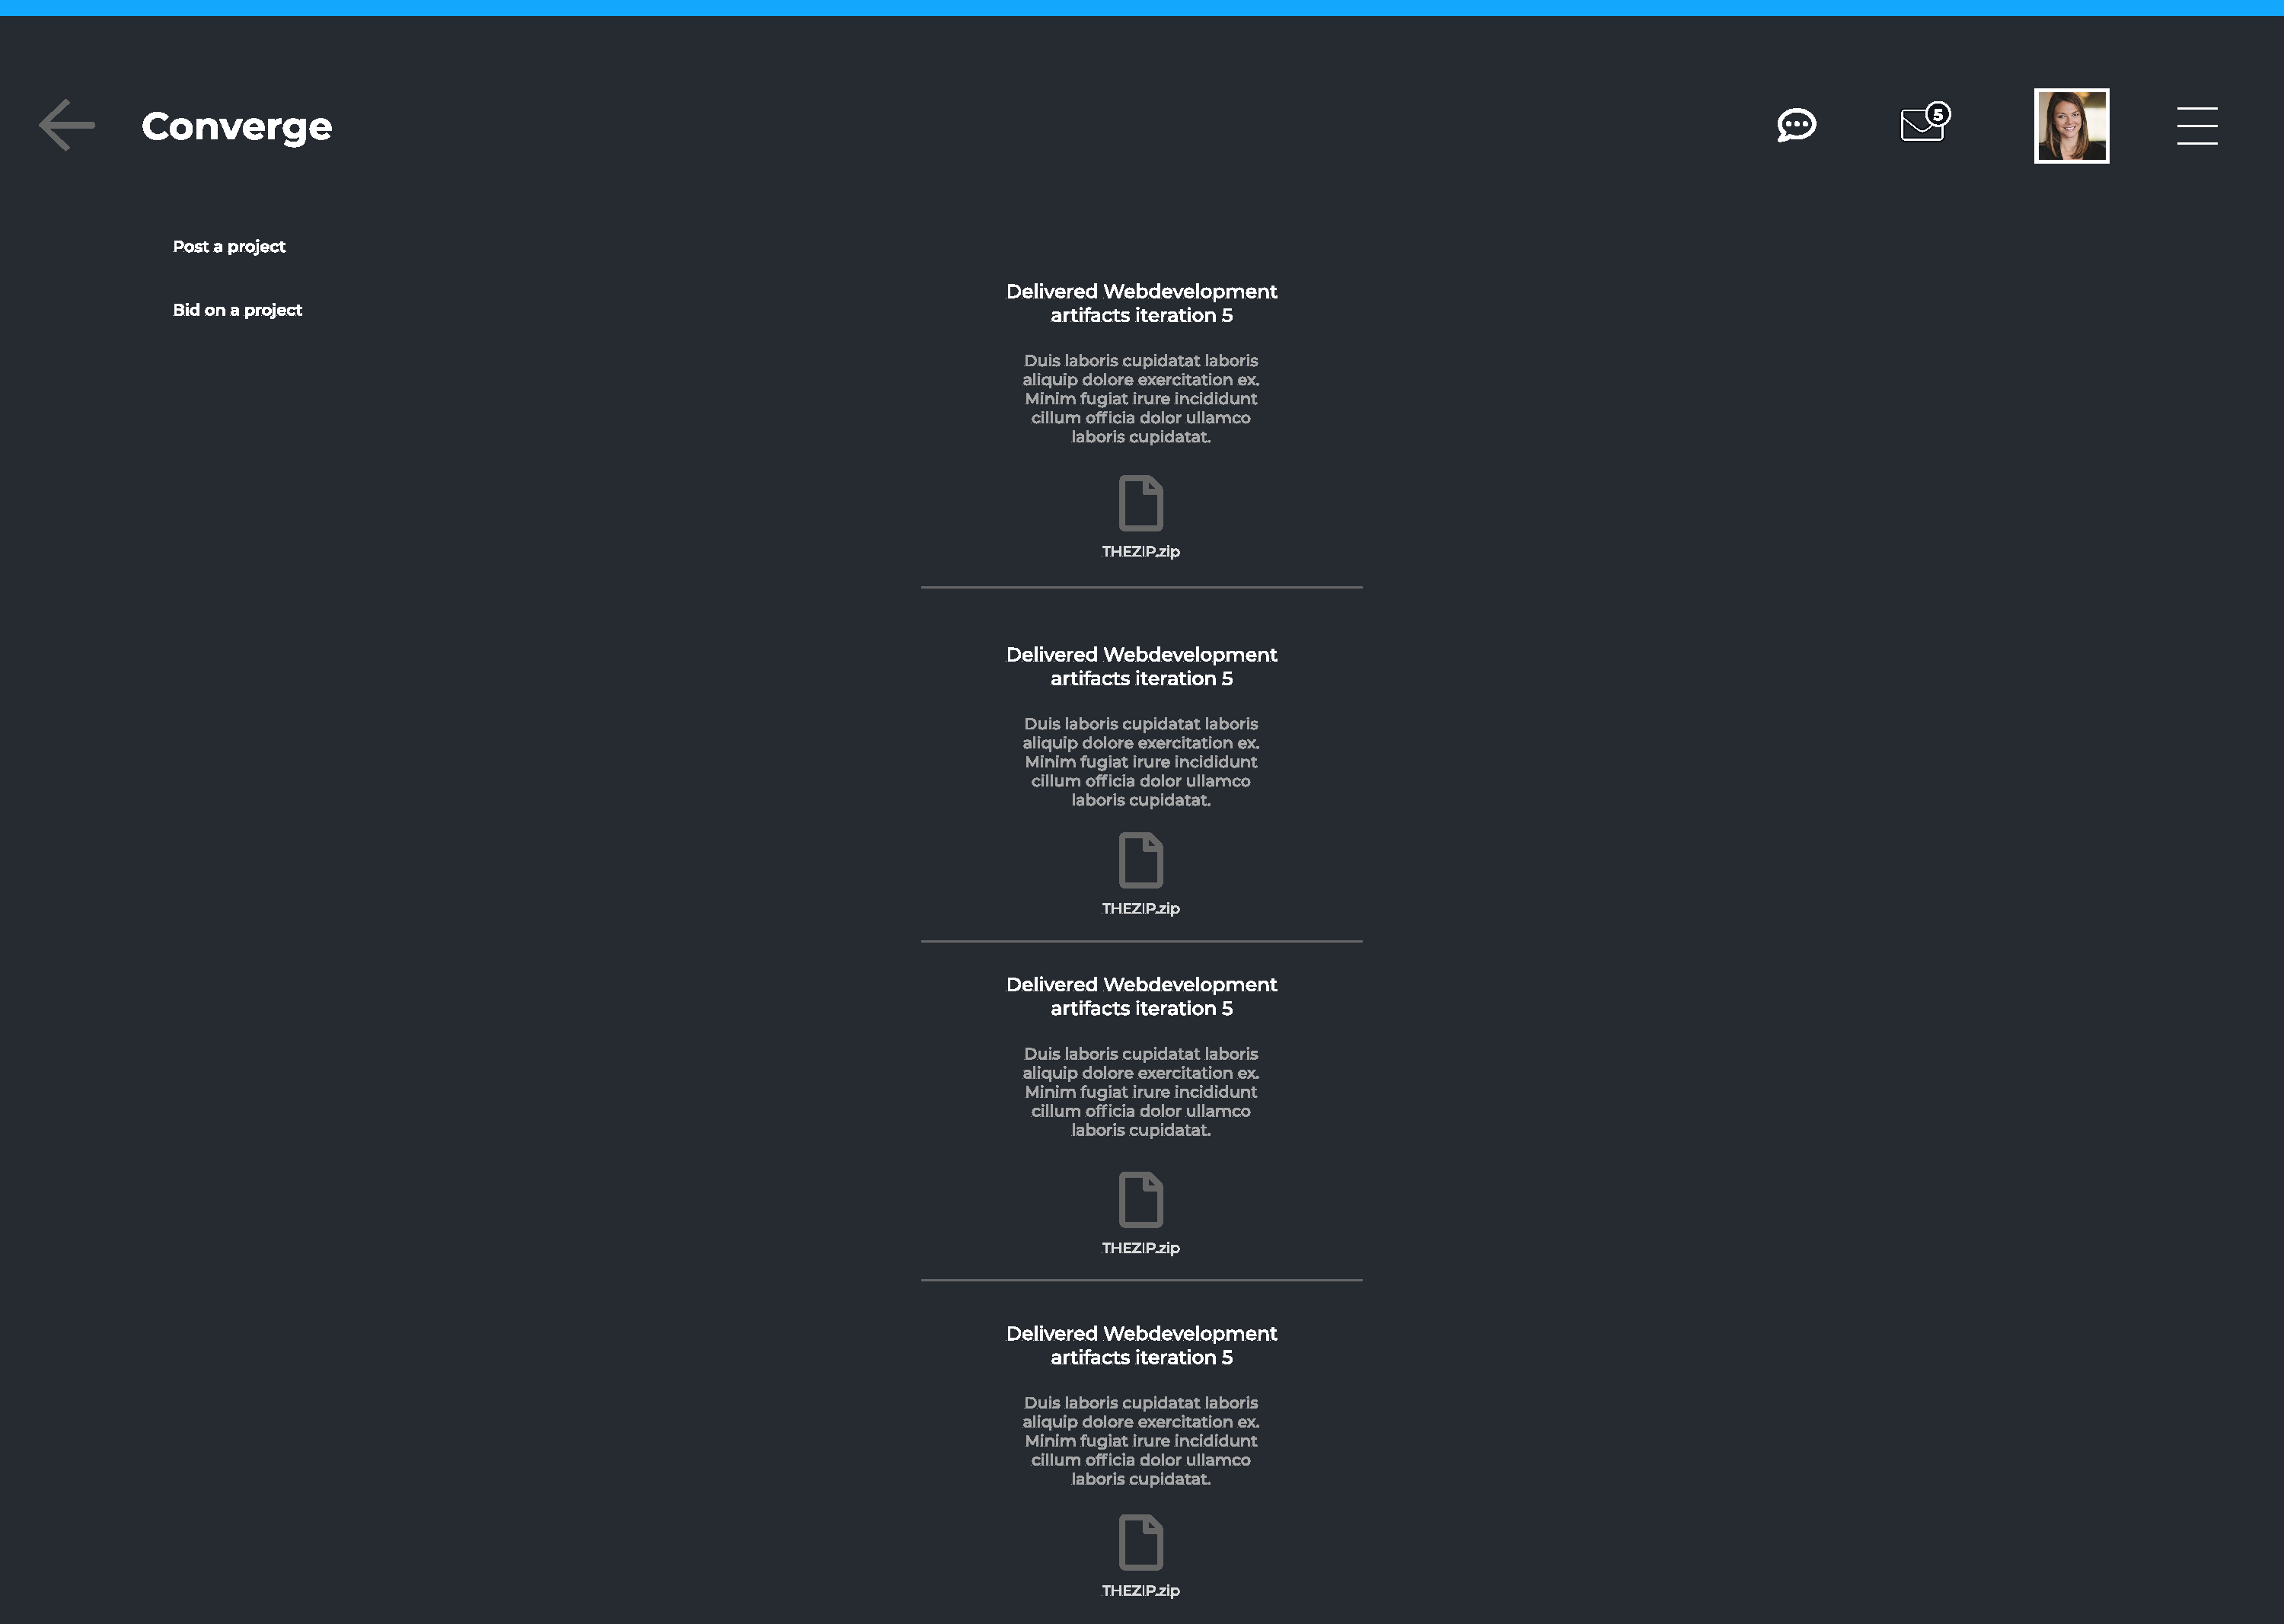
\includegraphics[width=0.6\textwidth]{system-interface-pic/Dashboard.pdf}
\caption{Viser dashboard side}
\label{fig:figure2}
\end{figure}

Når man er logget ind på Converge platformen med et succesfuldt login, så bliver dashboard siden vist. Her har brugeren følgende mugligheder: oprette et projekt, byde på et projekt som ses på venstre side af figur 1.5,i midten ser brugeren en liste af de færdiggjort projekter, op øverst på navigations baren har brugeren muglighed for at kunne tilgå sin profil, chat siden, kan se hvis brugeren har fået notification, kan logge ud og tilgå personlige indstillinger.

\newpage
\begin{figure}[ht]
    \centering
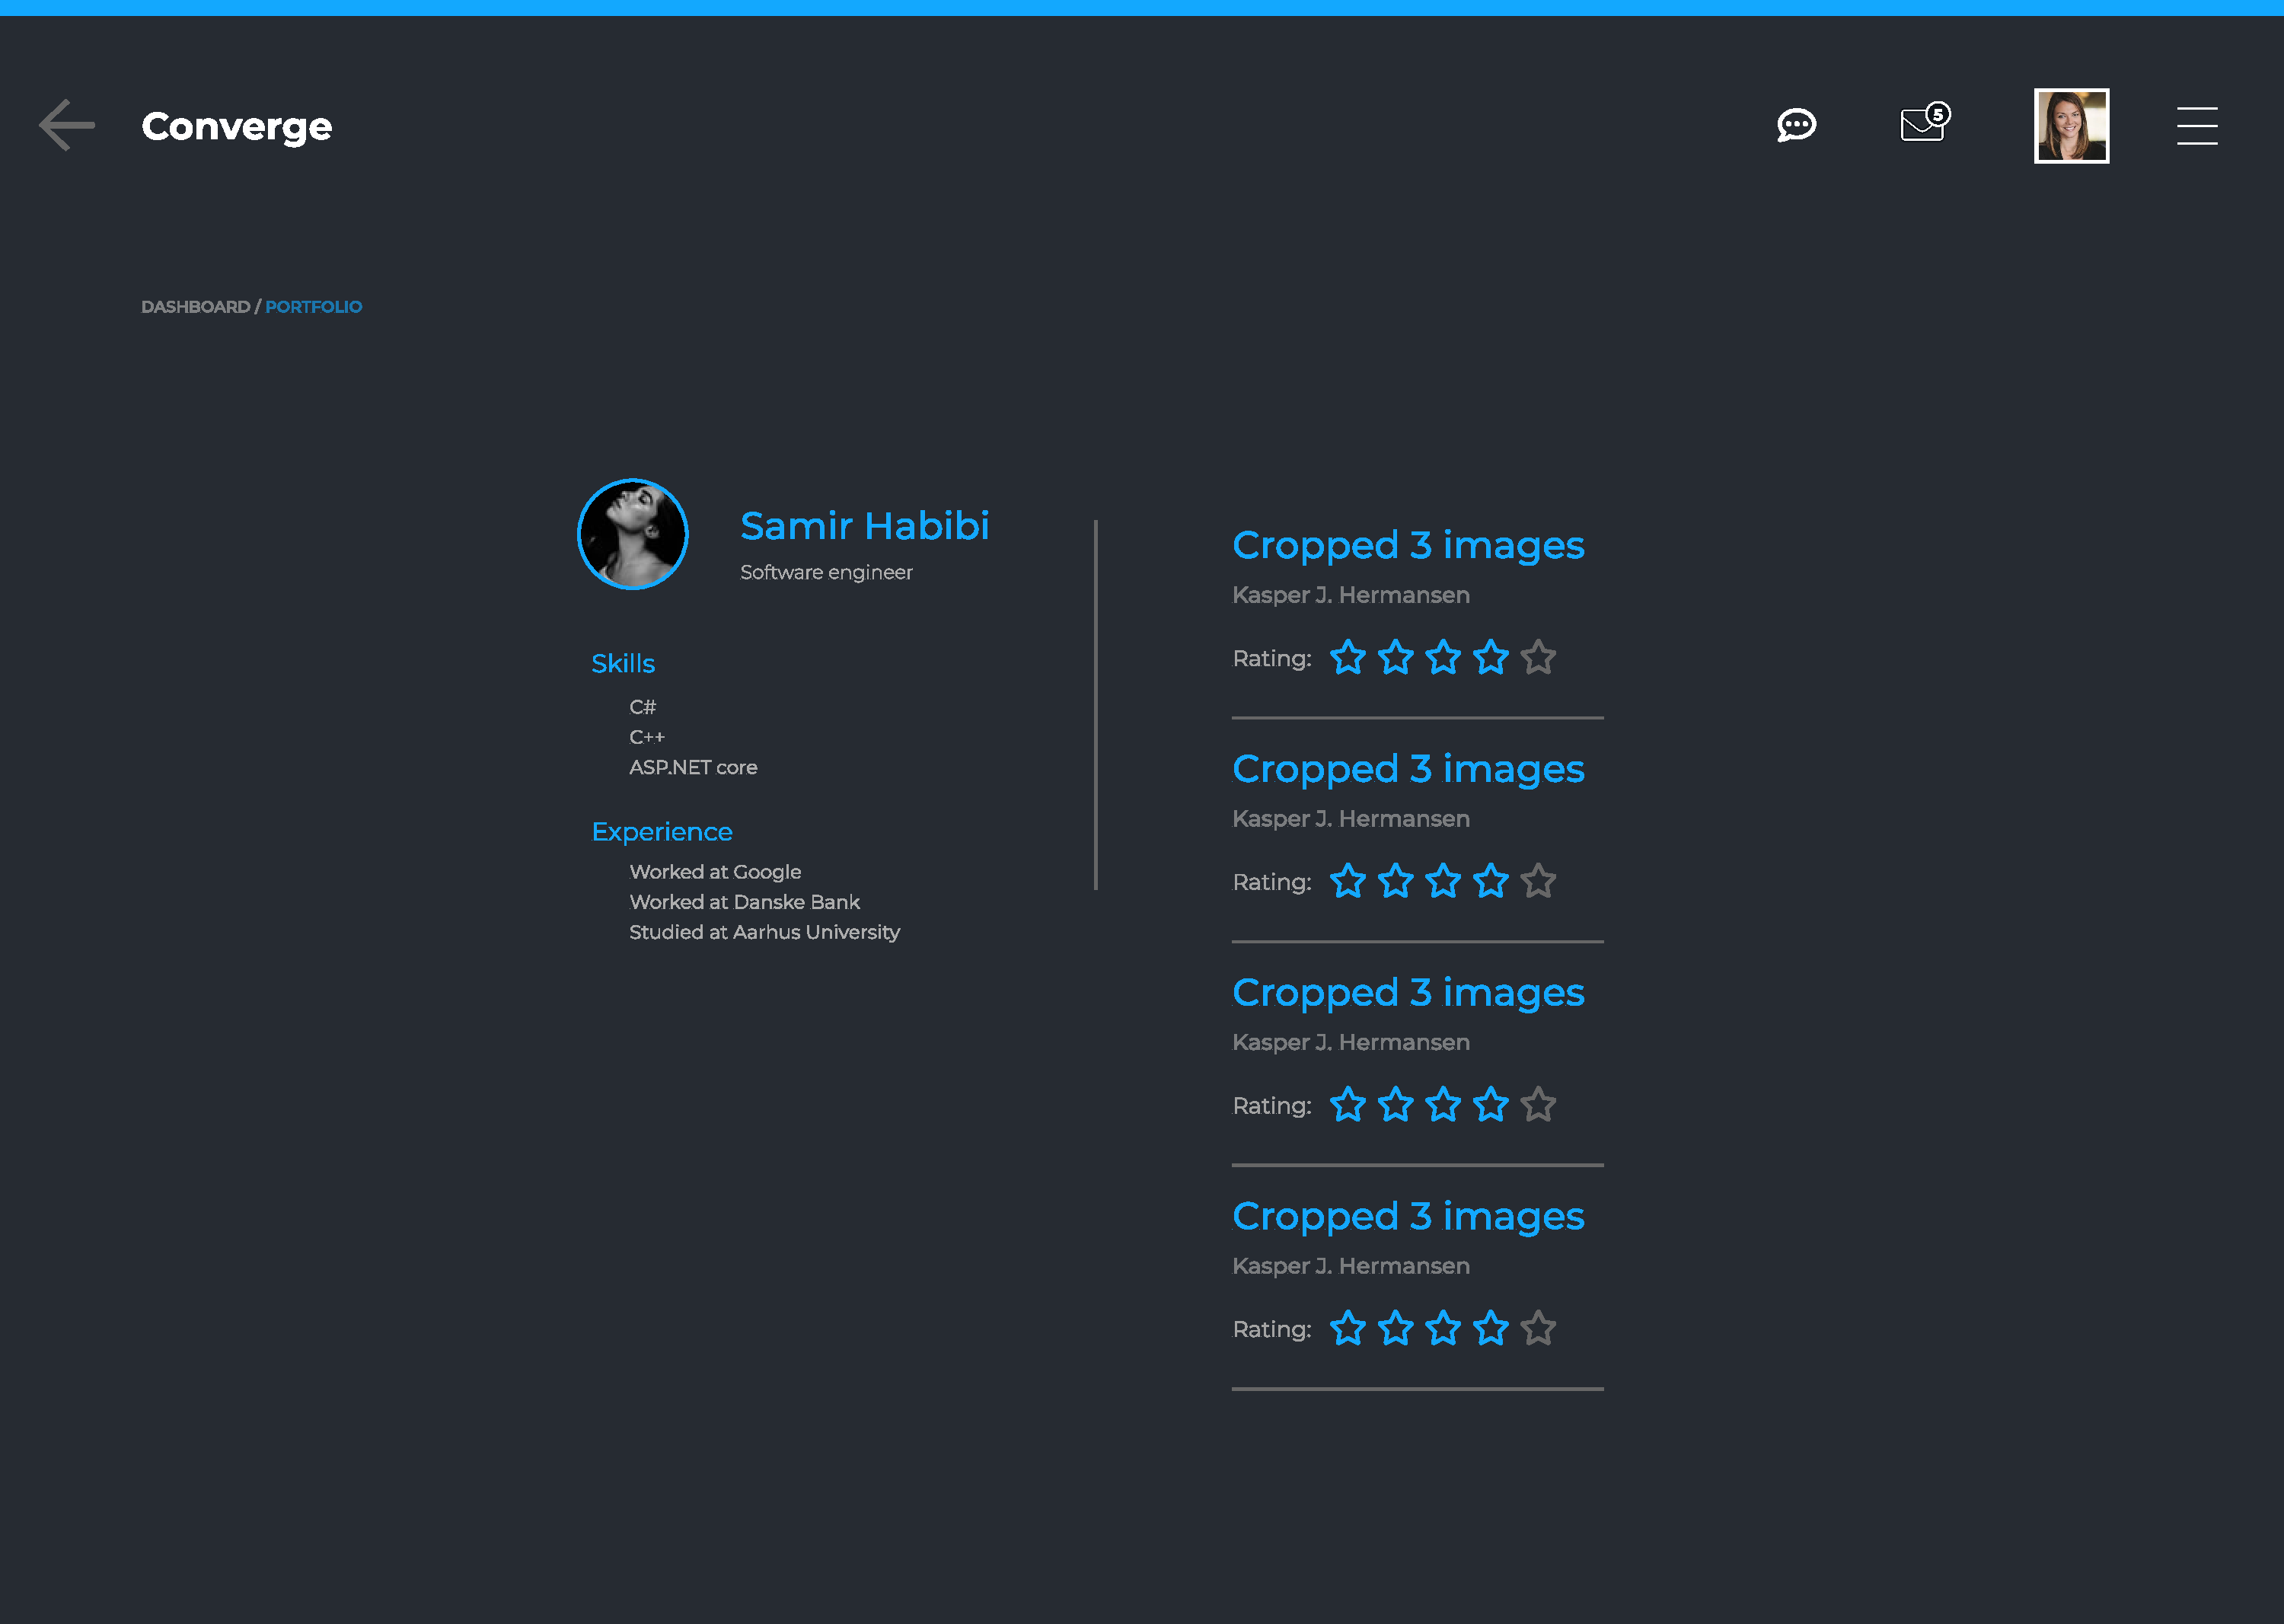
\includegraphics[width=0.6\textwidth]{system-interface-pic/Portfolio.pdf}
\caption{Viser profil side}
\label{fig:figure2}
\end{figure}

På figur 1.6 ses profil siden, her har brugeren muglighed for at tilføje sine personlige kompetencer og erfaring. Derudover vil der også være muglighed for bruger at kunne se de færdiggjorte projekter og hvordan de er blevet bedømt. 

\begin{figure}[ht]
    \centering
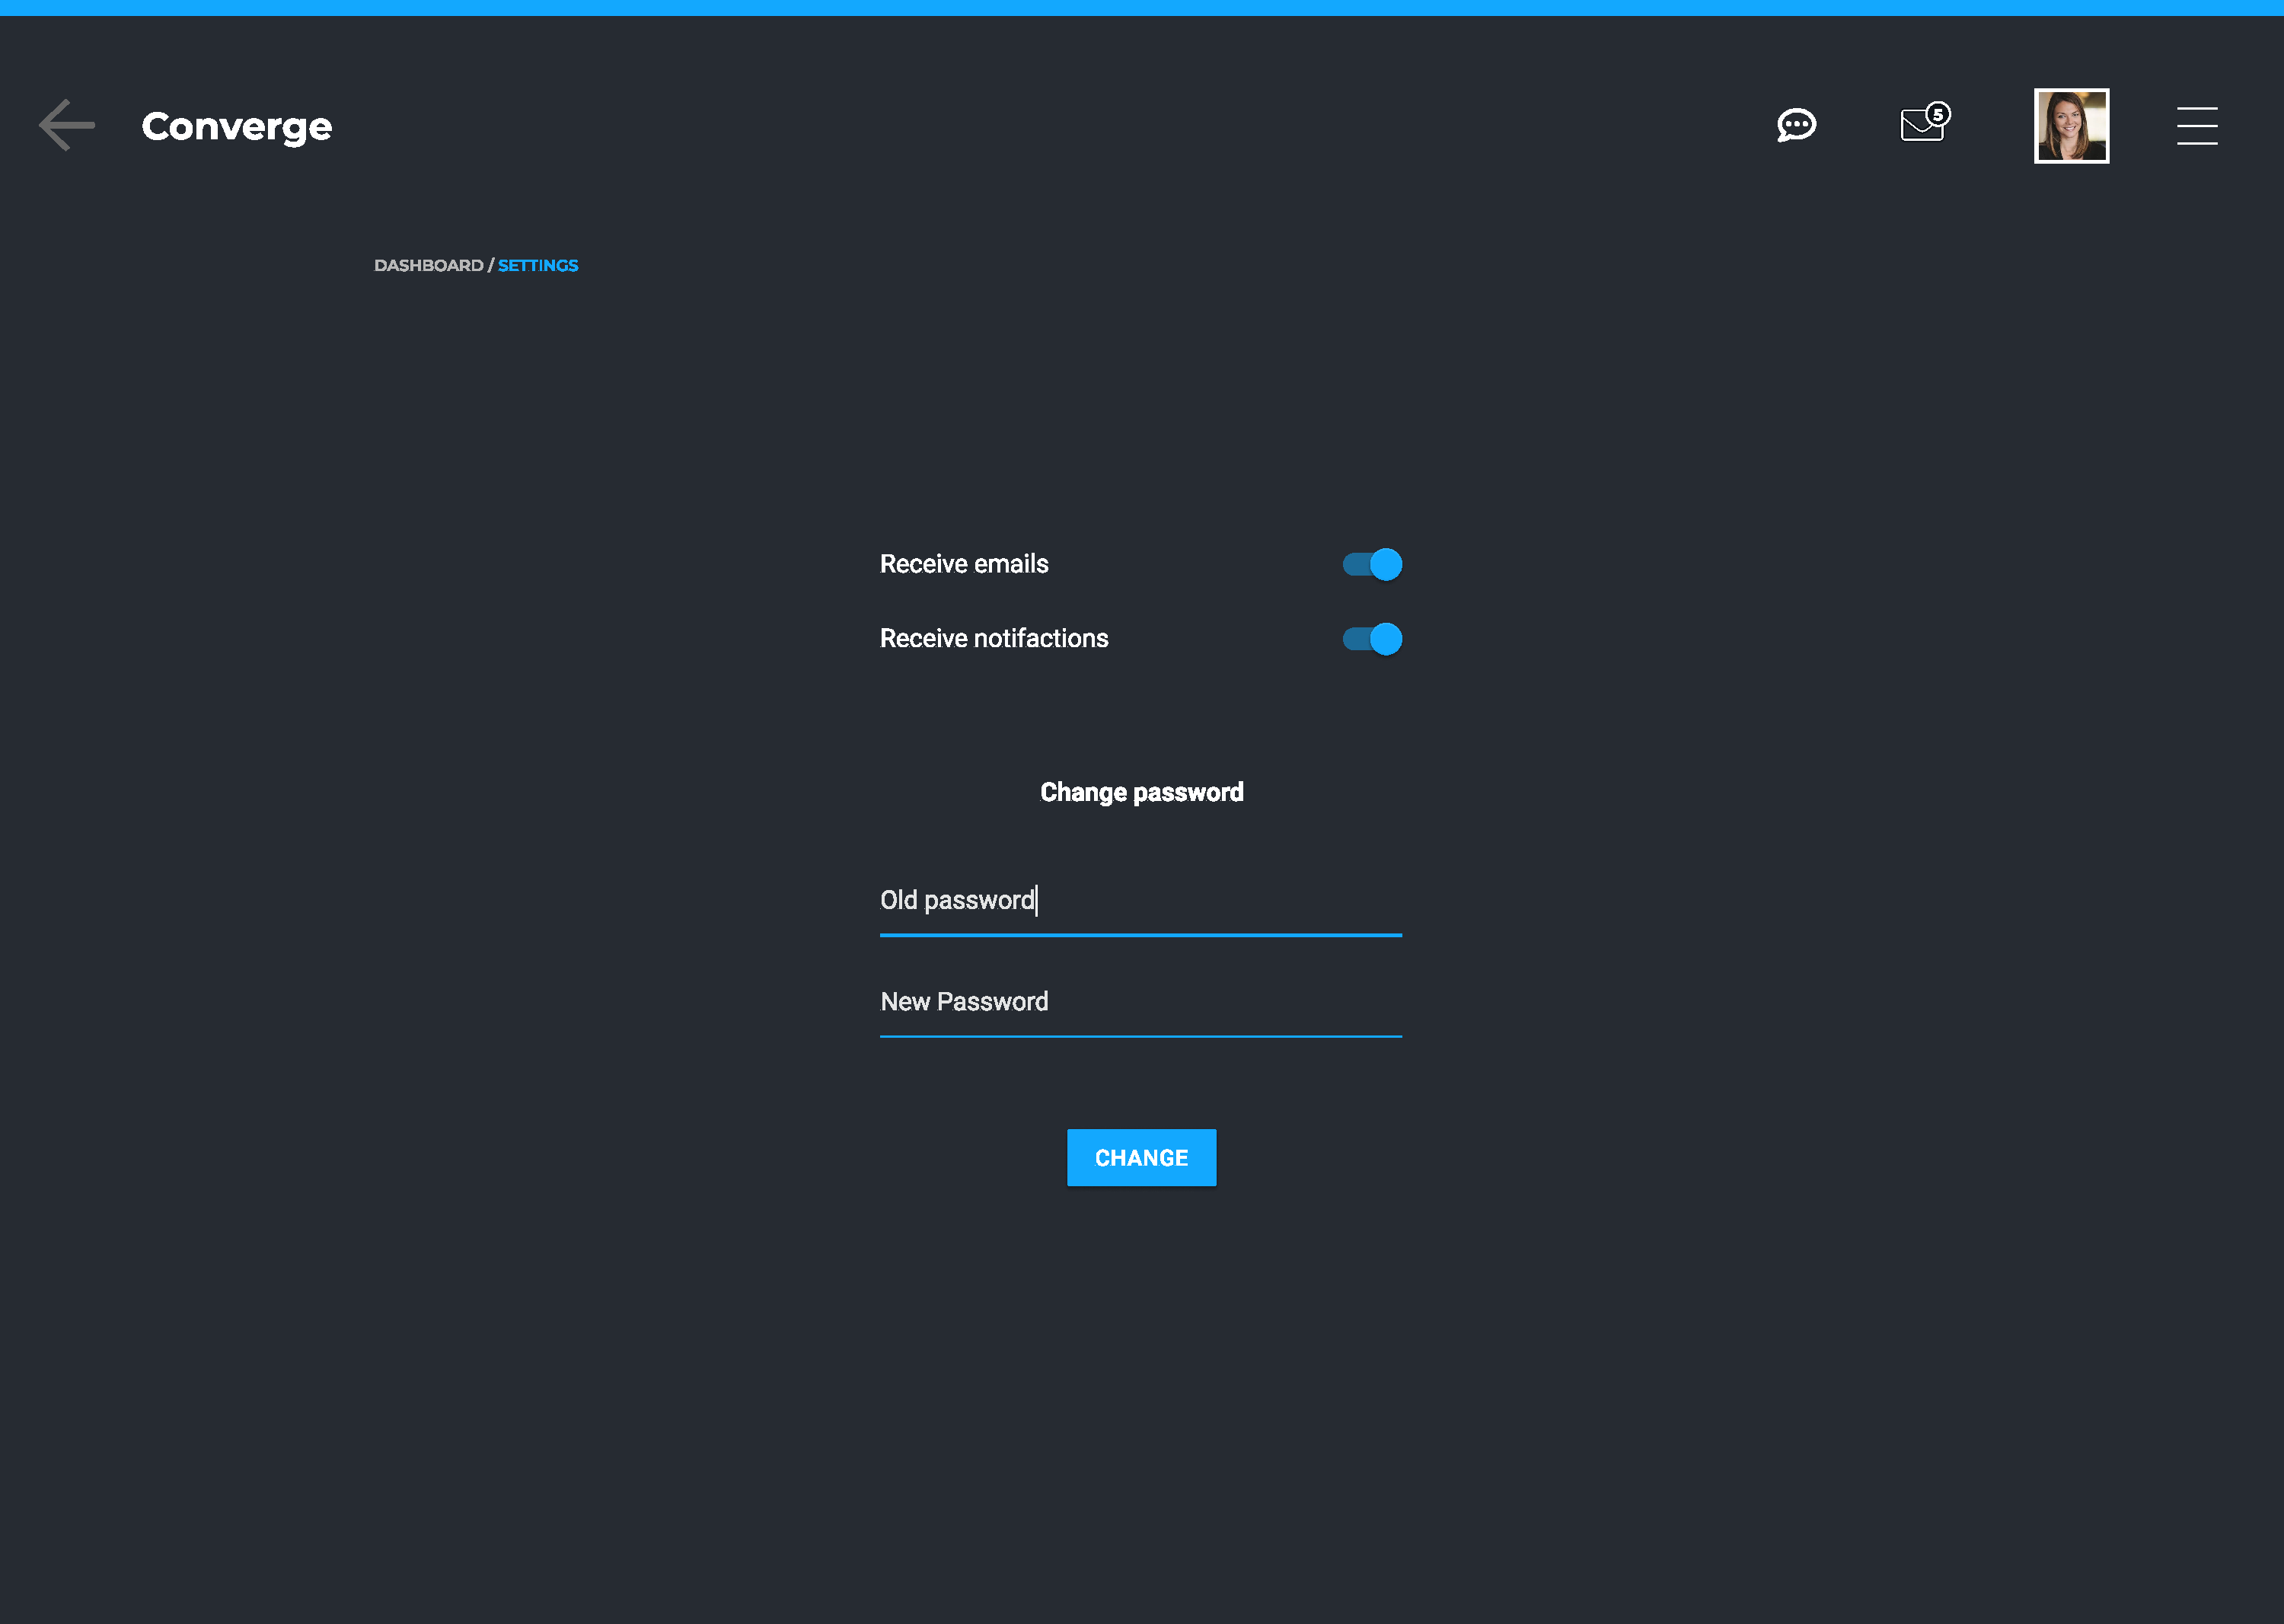
\includegraphics[width=0.6\textwidth]{system-interface-pic/Settings.pdf}
\caption{Viser indstilling side}
\label{fig:figure2}
\end{figure}

På figur 1.7 ses instilling siden og brugeren kan fortage personlige ændring efter eget ønske. Brugeren kan altså vælge og modtage email, notification eller ændre nuværende password.

\newpage
\begin{figure}[ht]
    \centering
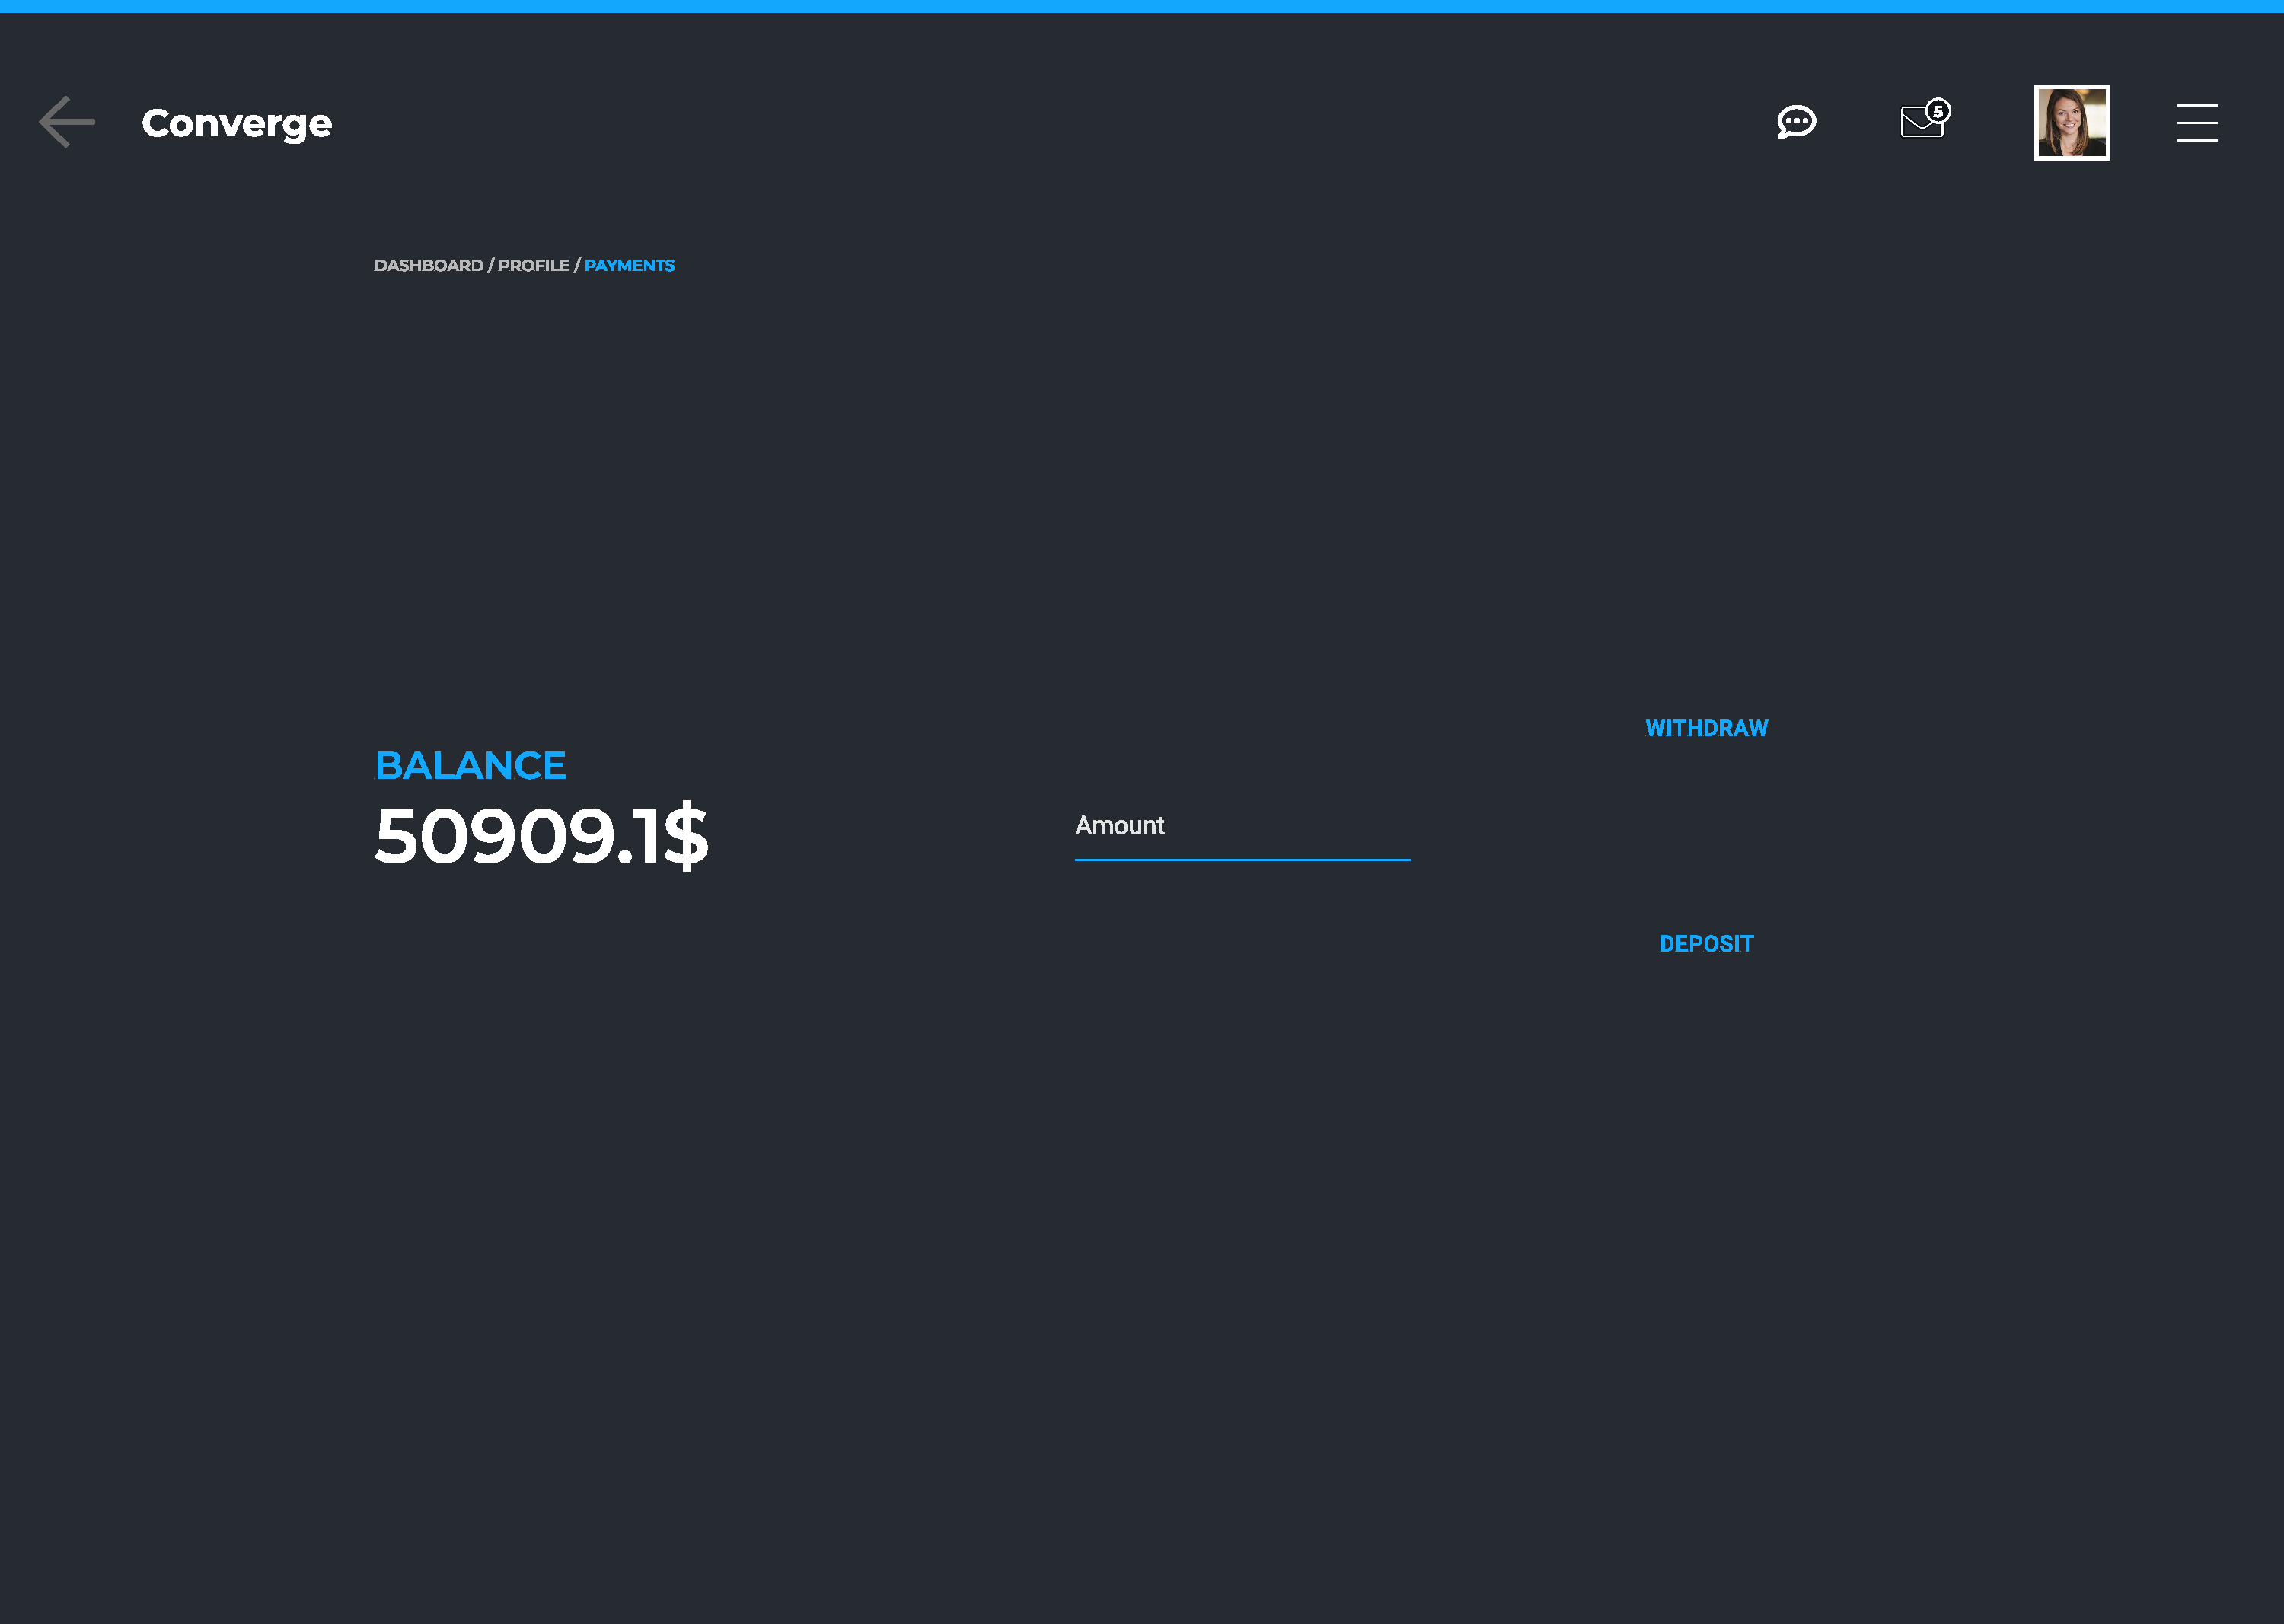
\includegraphics[width=0.6\textwidth]{system-interface-pic/Payments.pdf}
\caption{Viser betaling side}
\label{fig:figure2}
\end{figure}

Figur 1.8 viser betaling side, hvor brugeren har muglighed for at kunne se balancen på sin konto, modtage og udbetale penge. 

\begin{figure}[ht]
    \centering
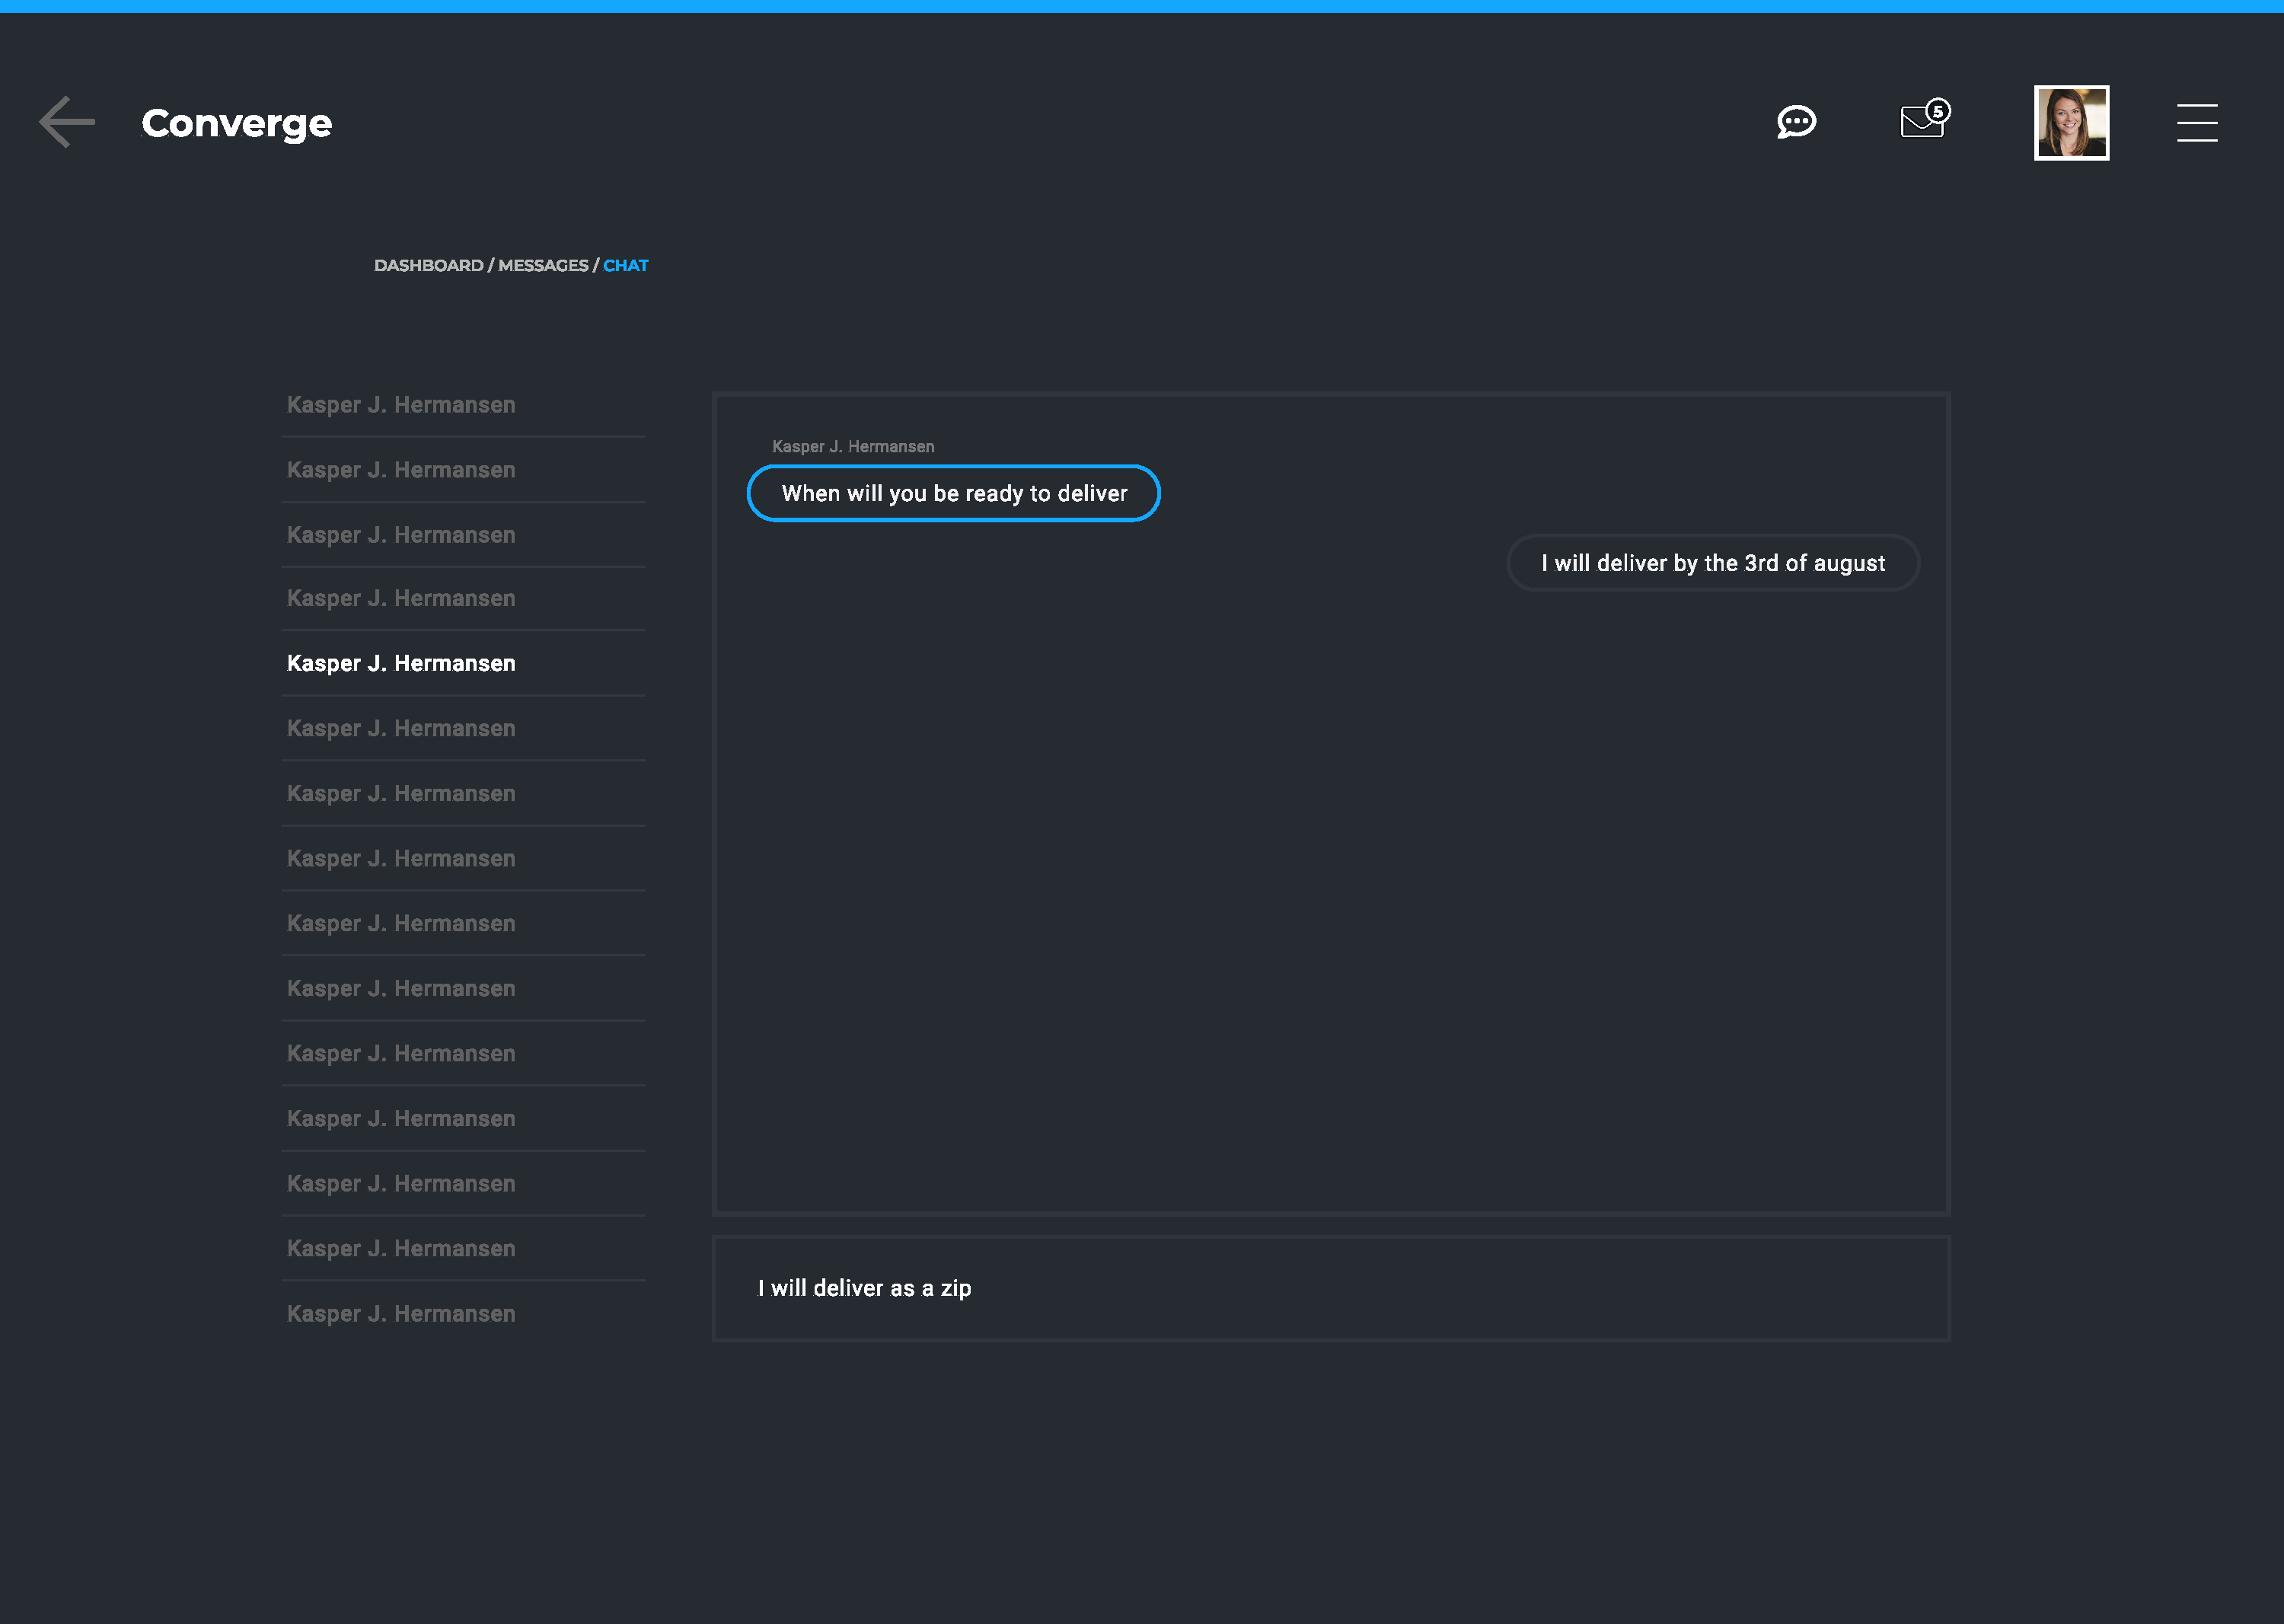
\includegraphics[width=0.6\textwidth]{system-interface-pic/Text-chat.pdf}
\caption{Viser chat side}
\label{fig:figure2}
\end{figure}

På figur 1.9 ses chat siden. Her kan brugeren send og modtage beskeder, derudover kan brugeren se liste over de forskellige kontakter på venstre side. 

\newpage
\begin{figure}[ht]
    \centering
\includegraphics[width=0.6\textwidth]{system-interface-pic/Video-chat.pdf}
\caption{Viser video chat side}
\label{fig:figure2}
\end{figure}
Figur 1.10 viser video chat, som brugeren kan benytte til at have direkte kontakt med andre brugere af Converge platformen. 

\begin{figure}[ht]
    \centering
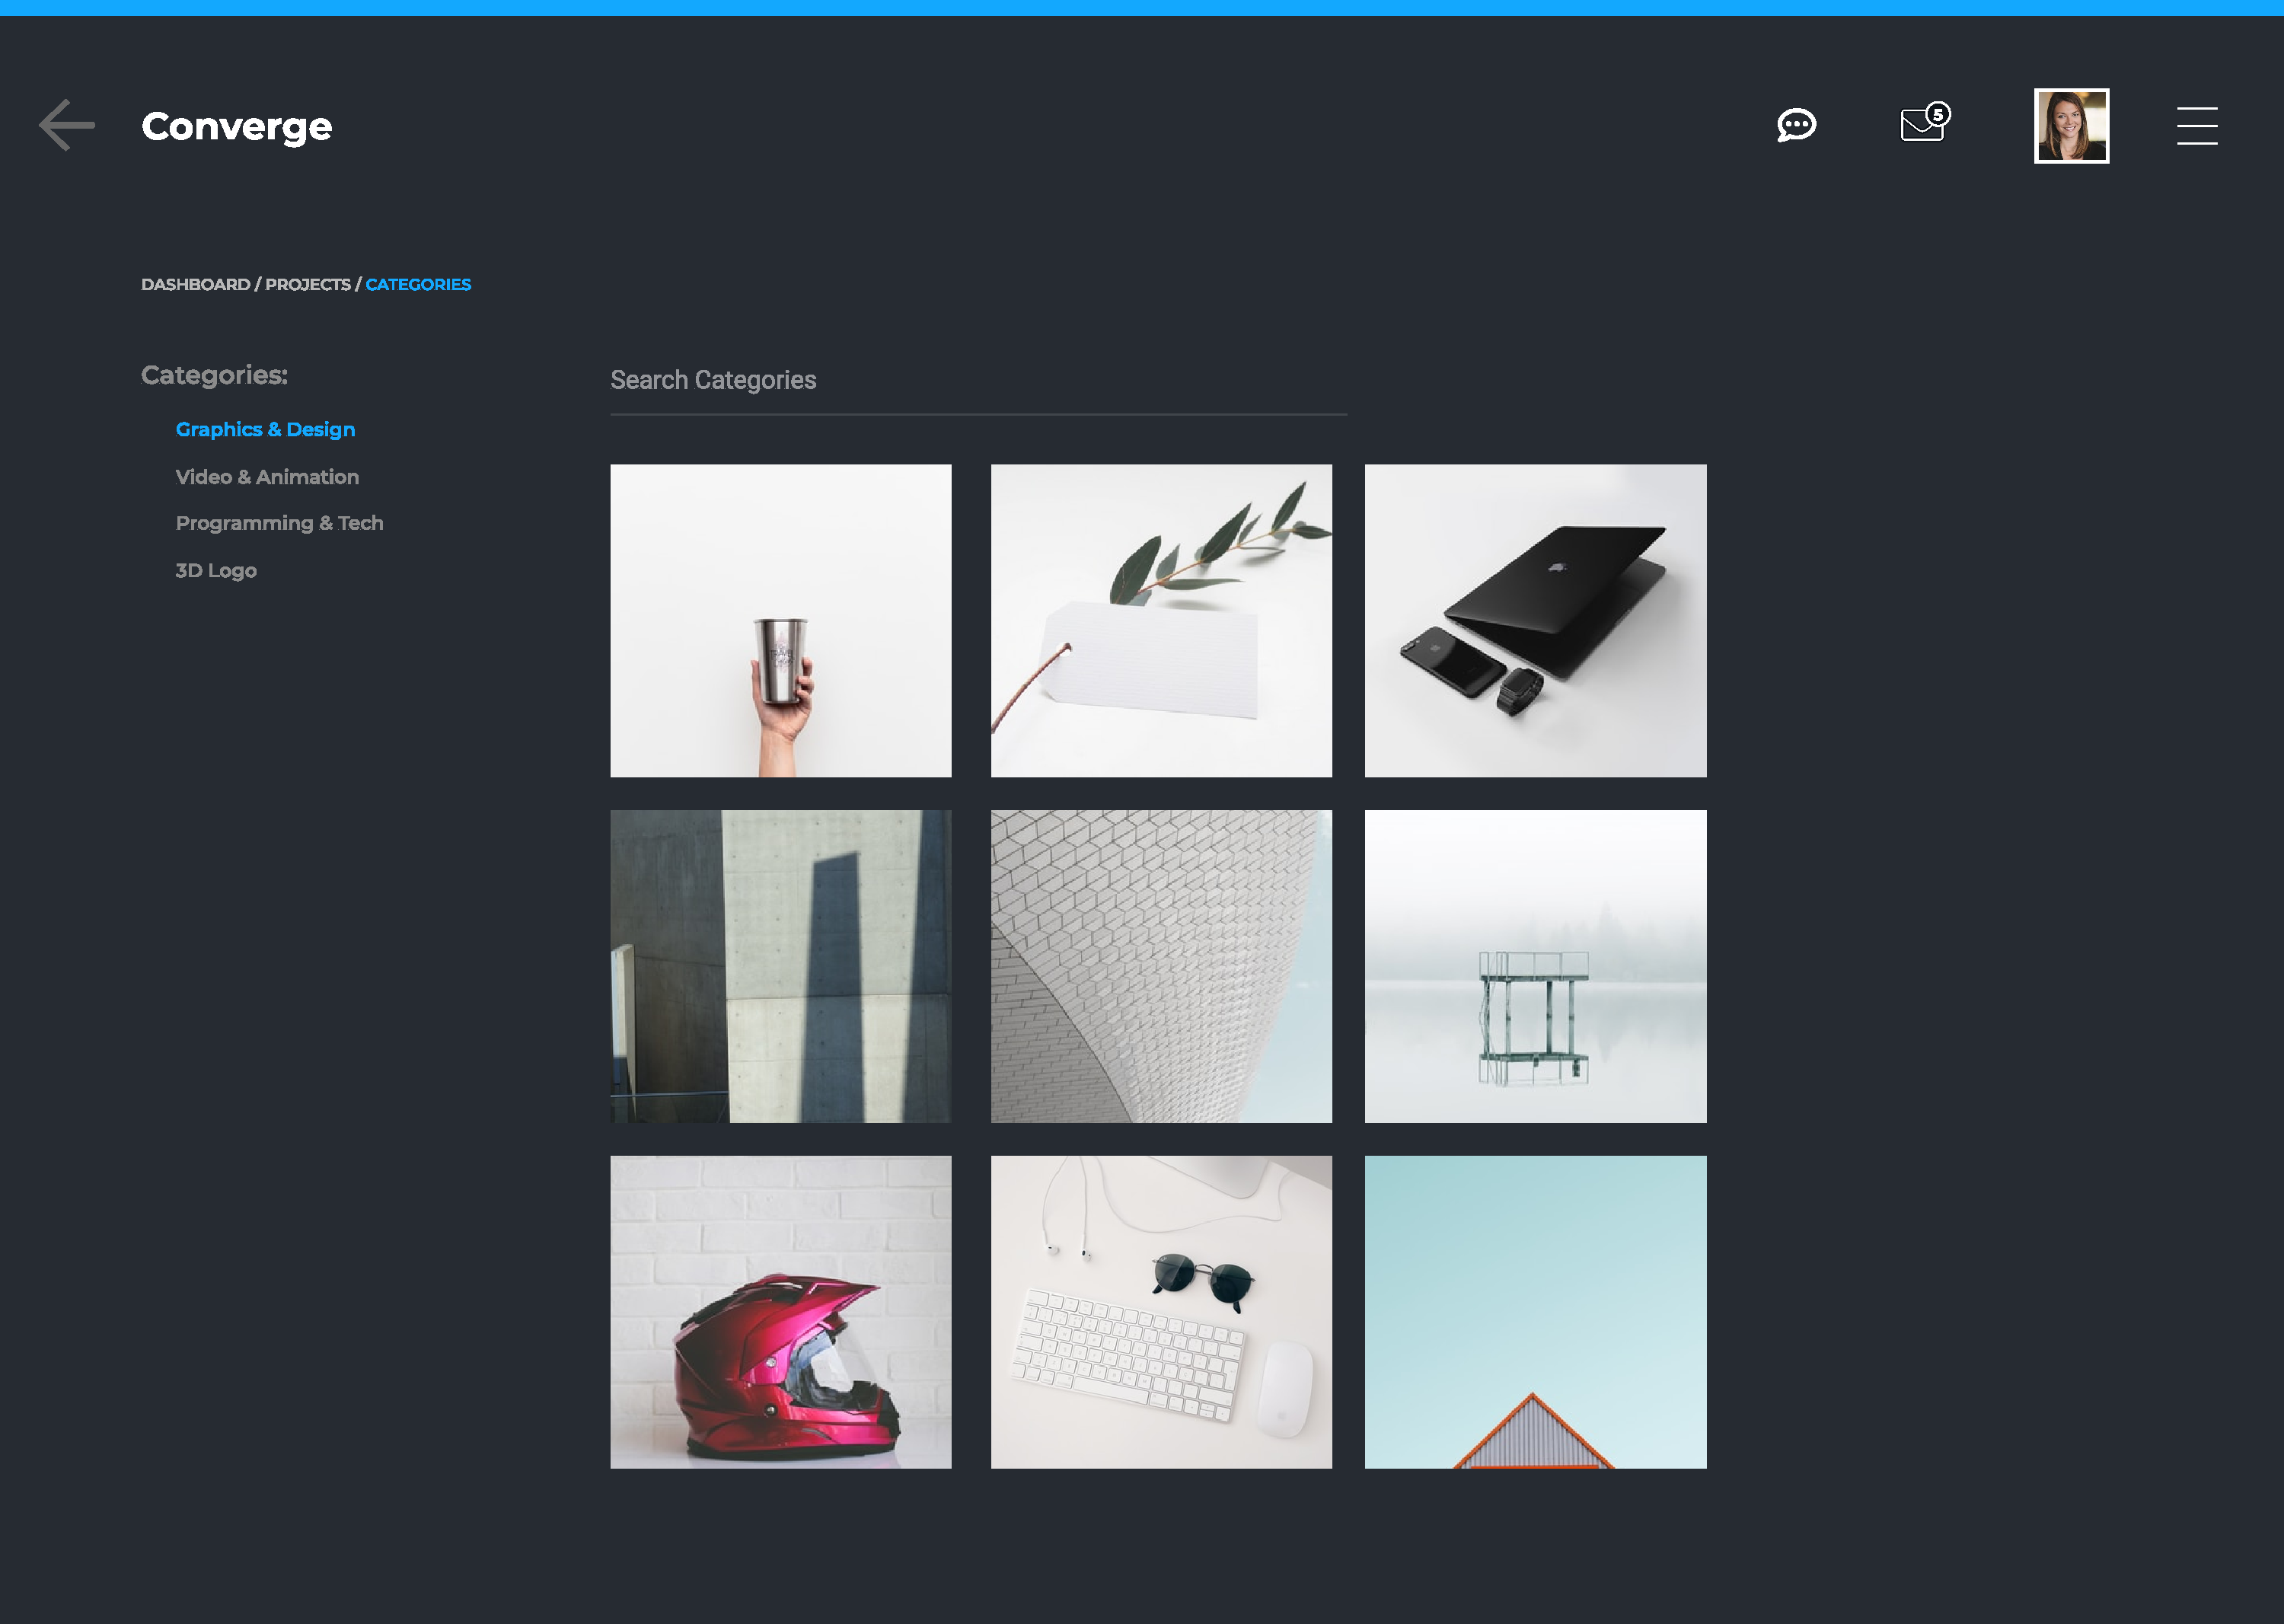
\includegraphics[width=0.6\textwidth]{system-interface-pic/Categories.pdf}
\caption{Viser kategori side}
\label{fig:figure2}
\end{figure}

Kategori siden, som ses på figur 1.11, her har brugeren muglighed for at vælge en af de forskellige kategorier, derudover kan brugeren også søge efter en specifik kategori.

\newpage
\begin{figure}[ht]
    \centering
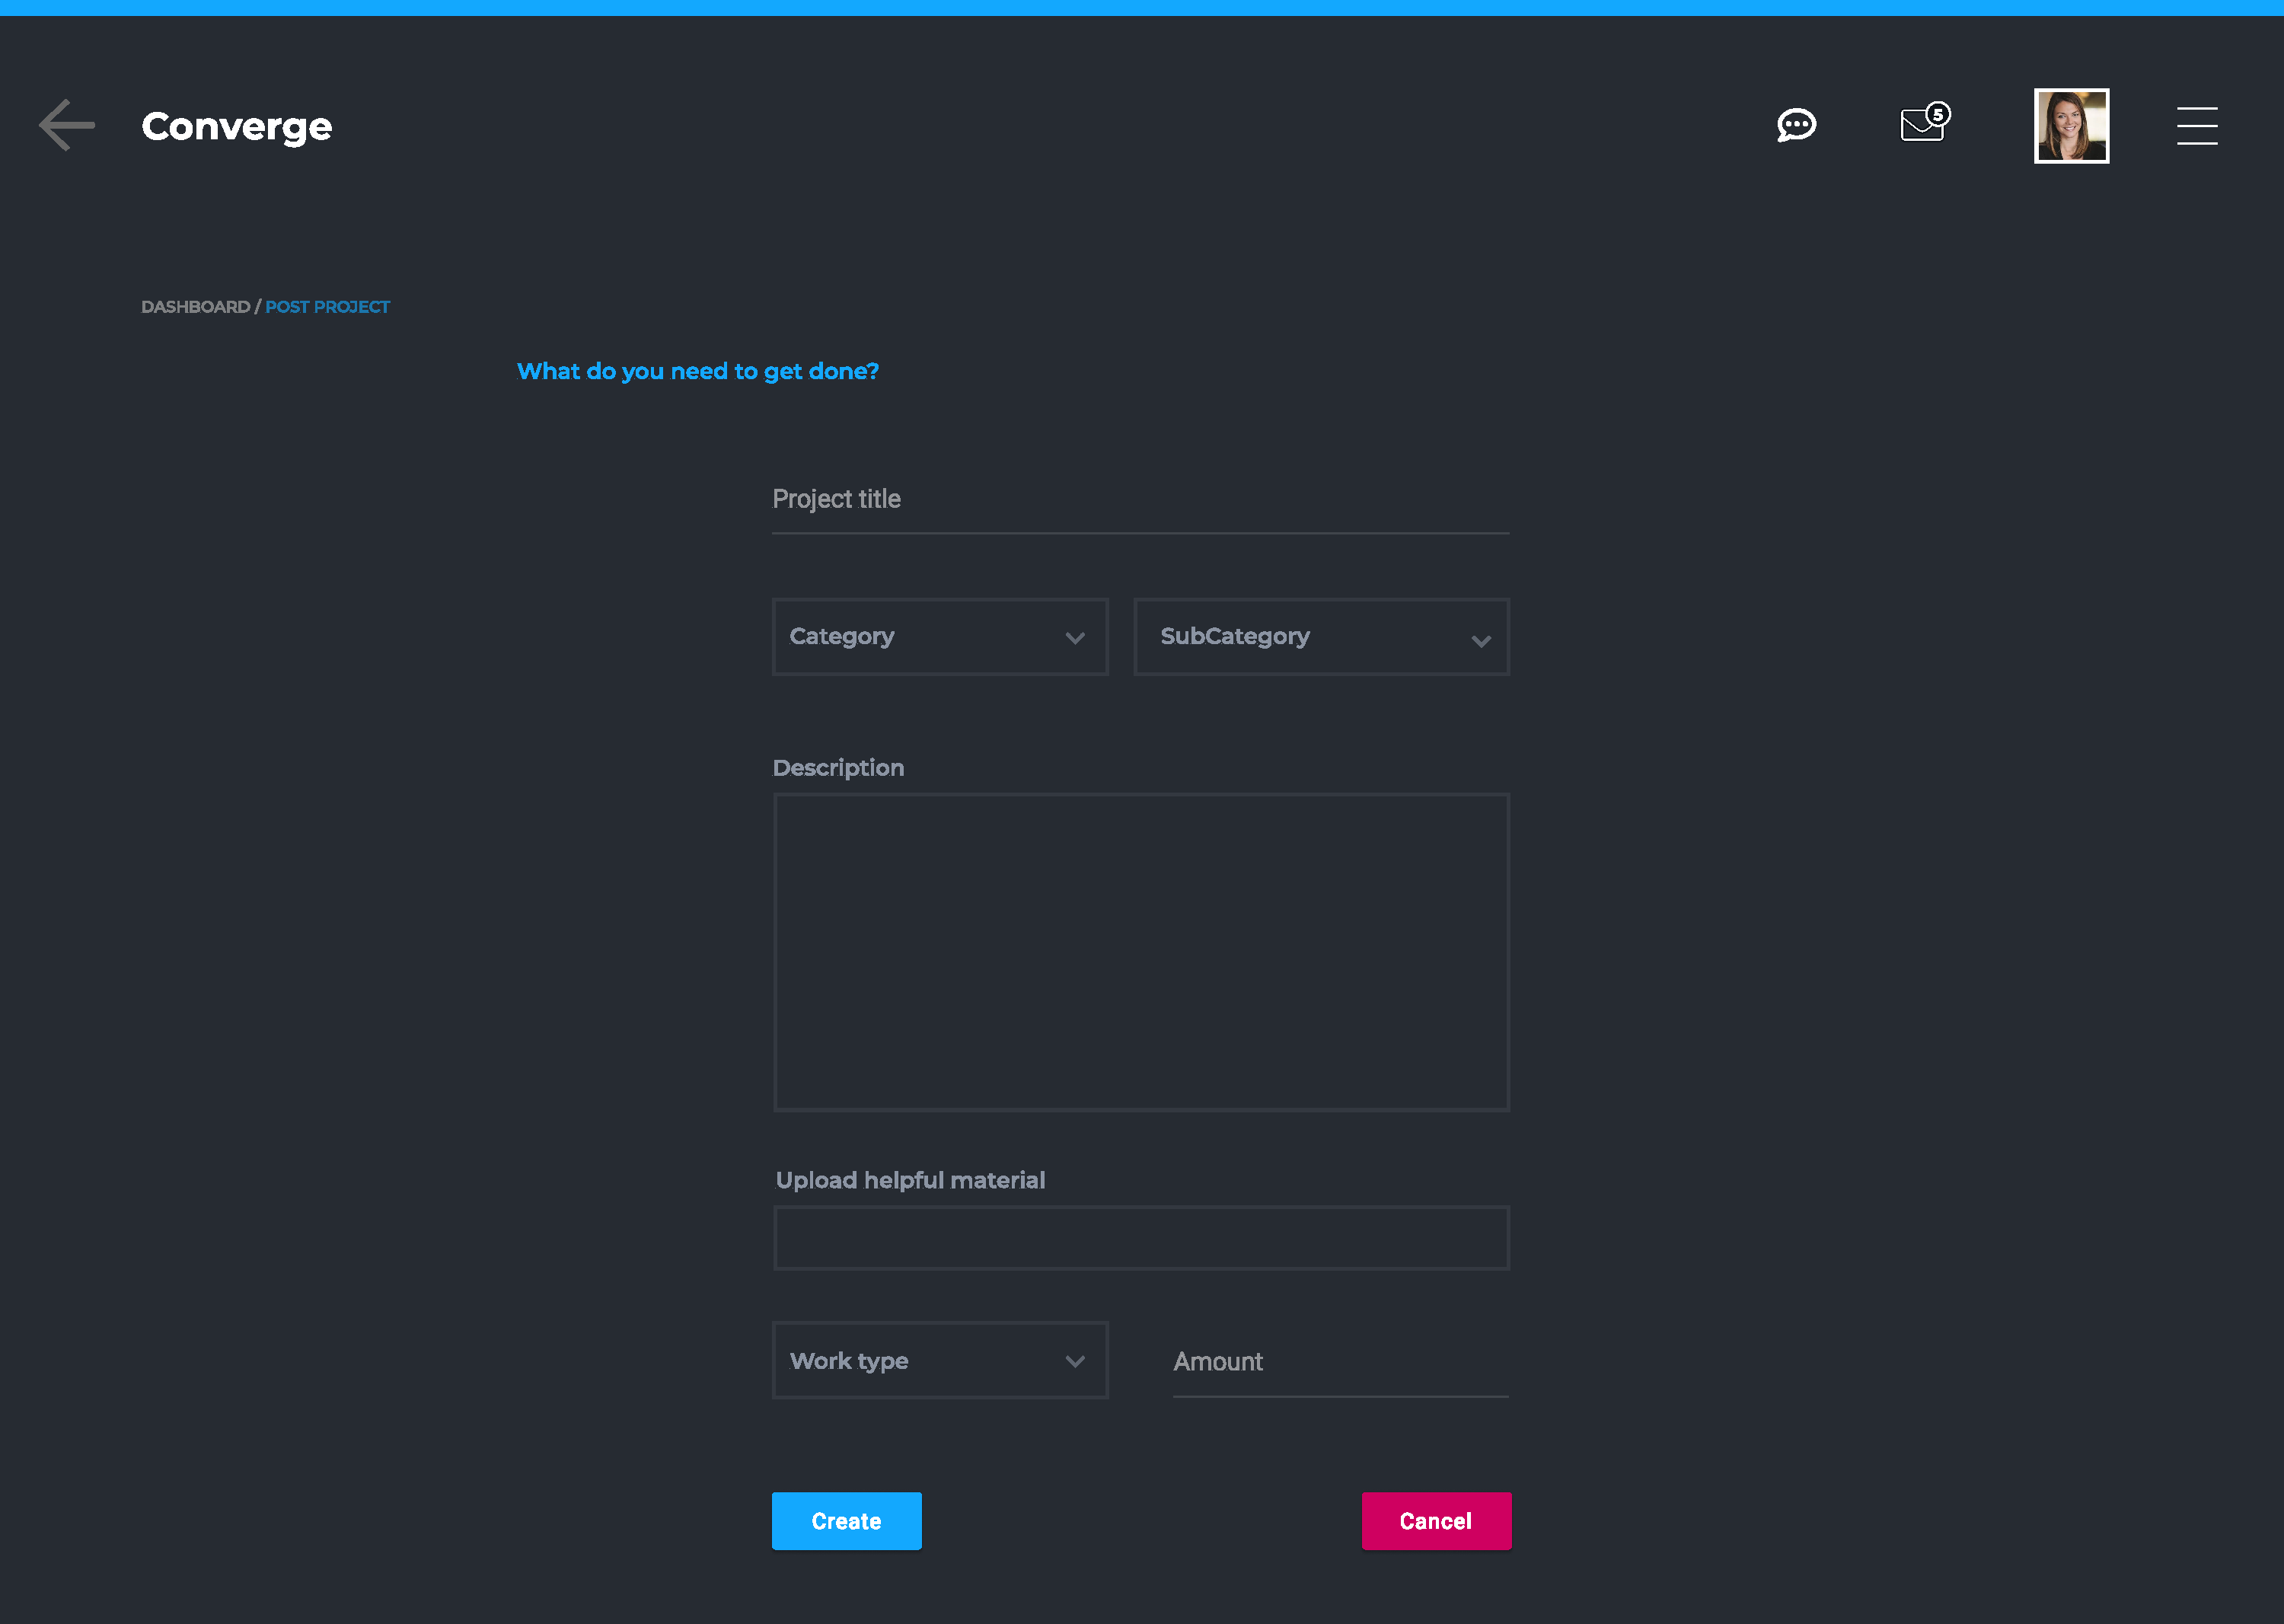
\includegraphics[width=0.6\textwidth]{system-interface-pic/Post-Project.pdf}
\caption{Viser hvor brugeren kan oprette et projekt}
\label{fig:figure2}
\end{figure}

Ovenstående figur viser siden, hvor brugeren har muglighed for at kunne oprette et projekt. 

\begin{figure}[ht]
    \centering
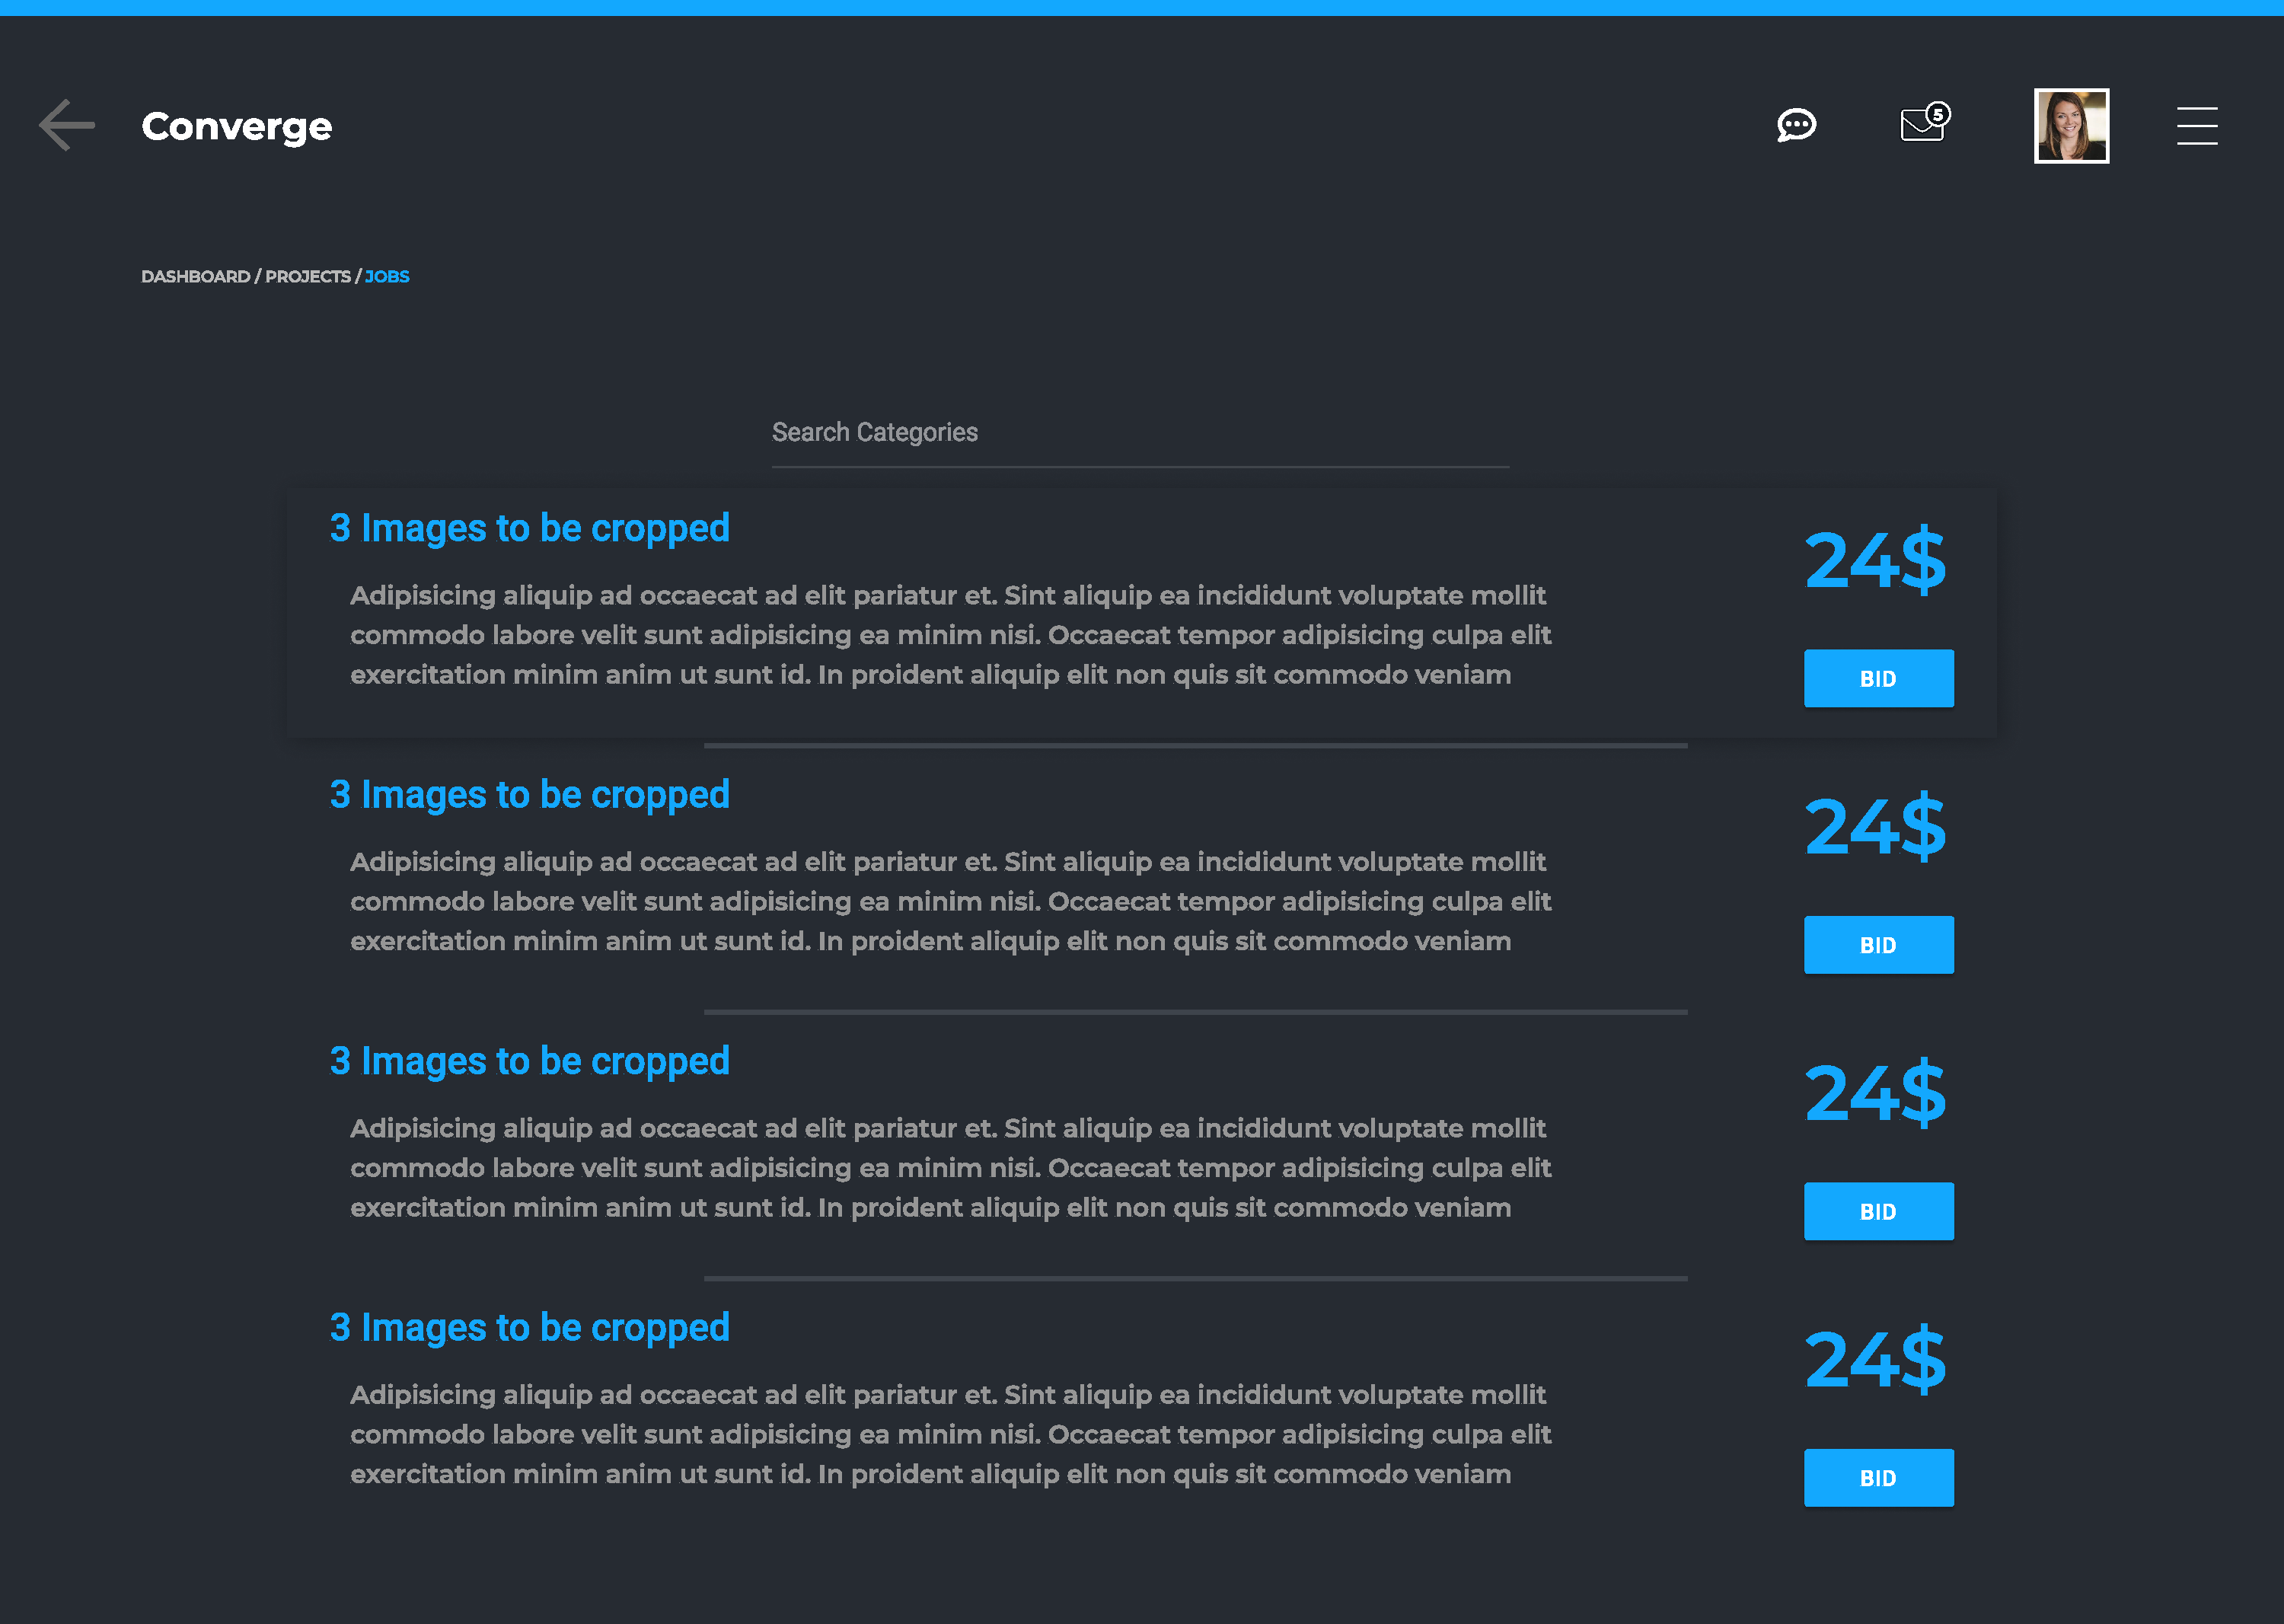
\includegraphics[width=0.6\textwidth]{system-interface-pic/Product-job.pdf}
\caption{Viser et oversigt over de tilgængelige projekter}
\label{fig:figure2}
\end{figure}

Figur 1.13 viser siden over de tilgængelige projekter, som brugeren har muglighed for at læse kort om projektets indhold. Hvis projektet fanger brugerens interesse, kan han/hun vælge og gå videre ved at trykke byd. 

\newpage
\begin{figure}[ht]
    \centering
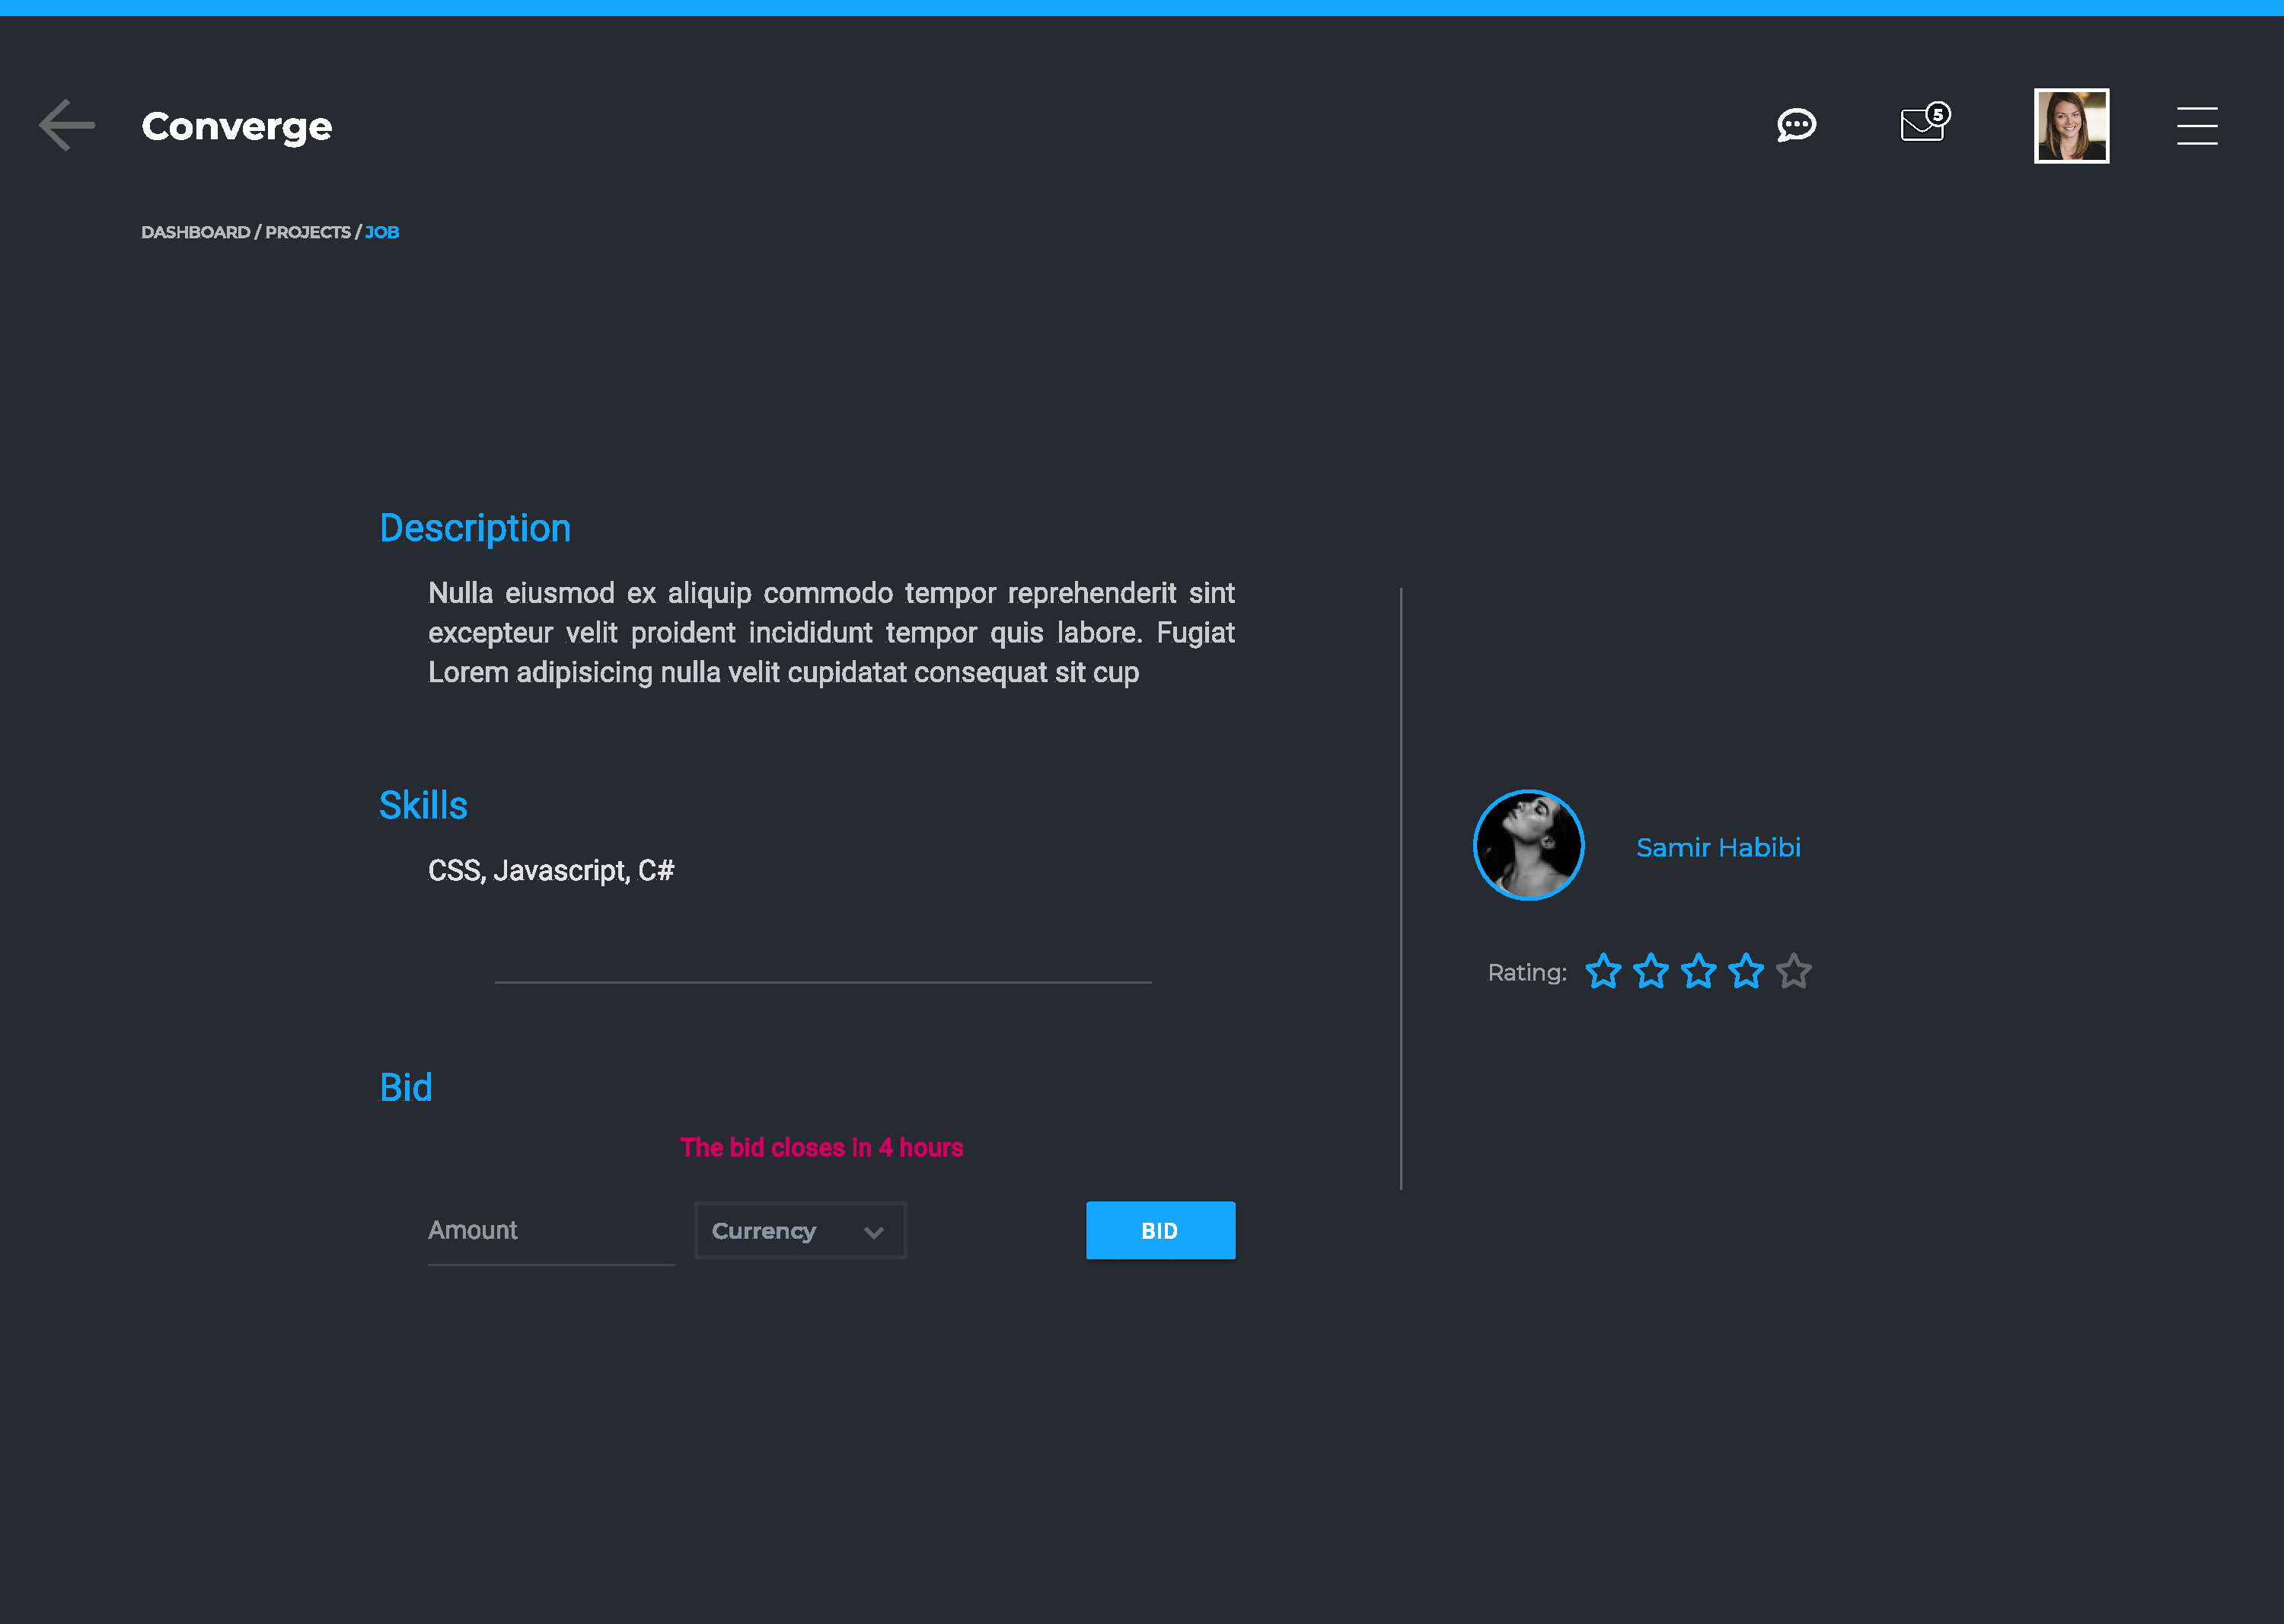
\includegraphics[width=0.6\textwidth]{system-interface-pic/Job.pdf}
\caption{Viser byde siden}
\label{fig:figure2}
\end{figure}

På figur 1.14 ses byde siden, her vil brugeren have muglighed for at kunne oprette et bud på det valgte projekt. På siden vil der også være projektets beskrivelse og hvilken færdigheder man skal have. 

\begin{figure}[ht]
    \centering
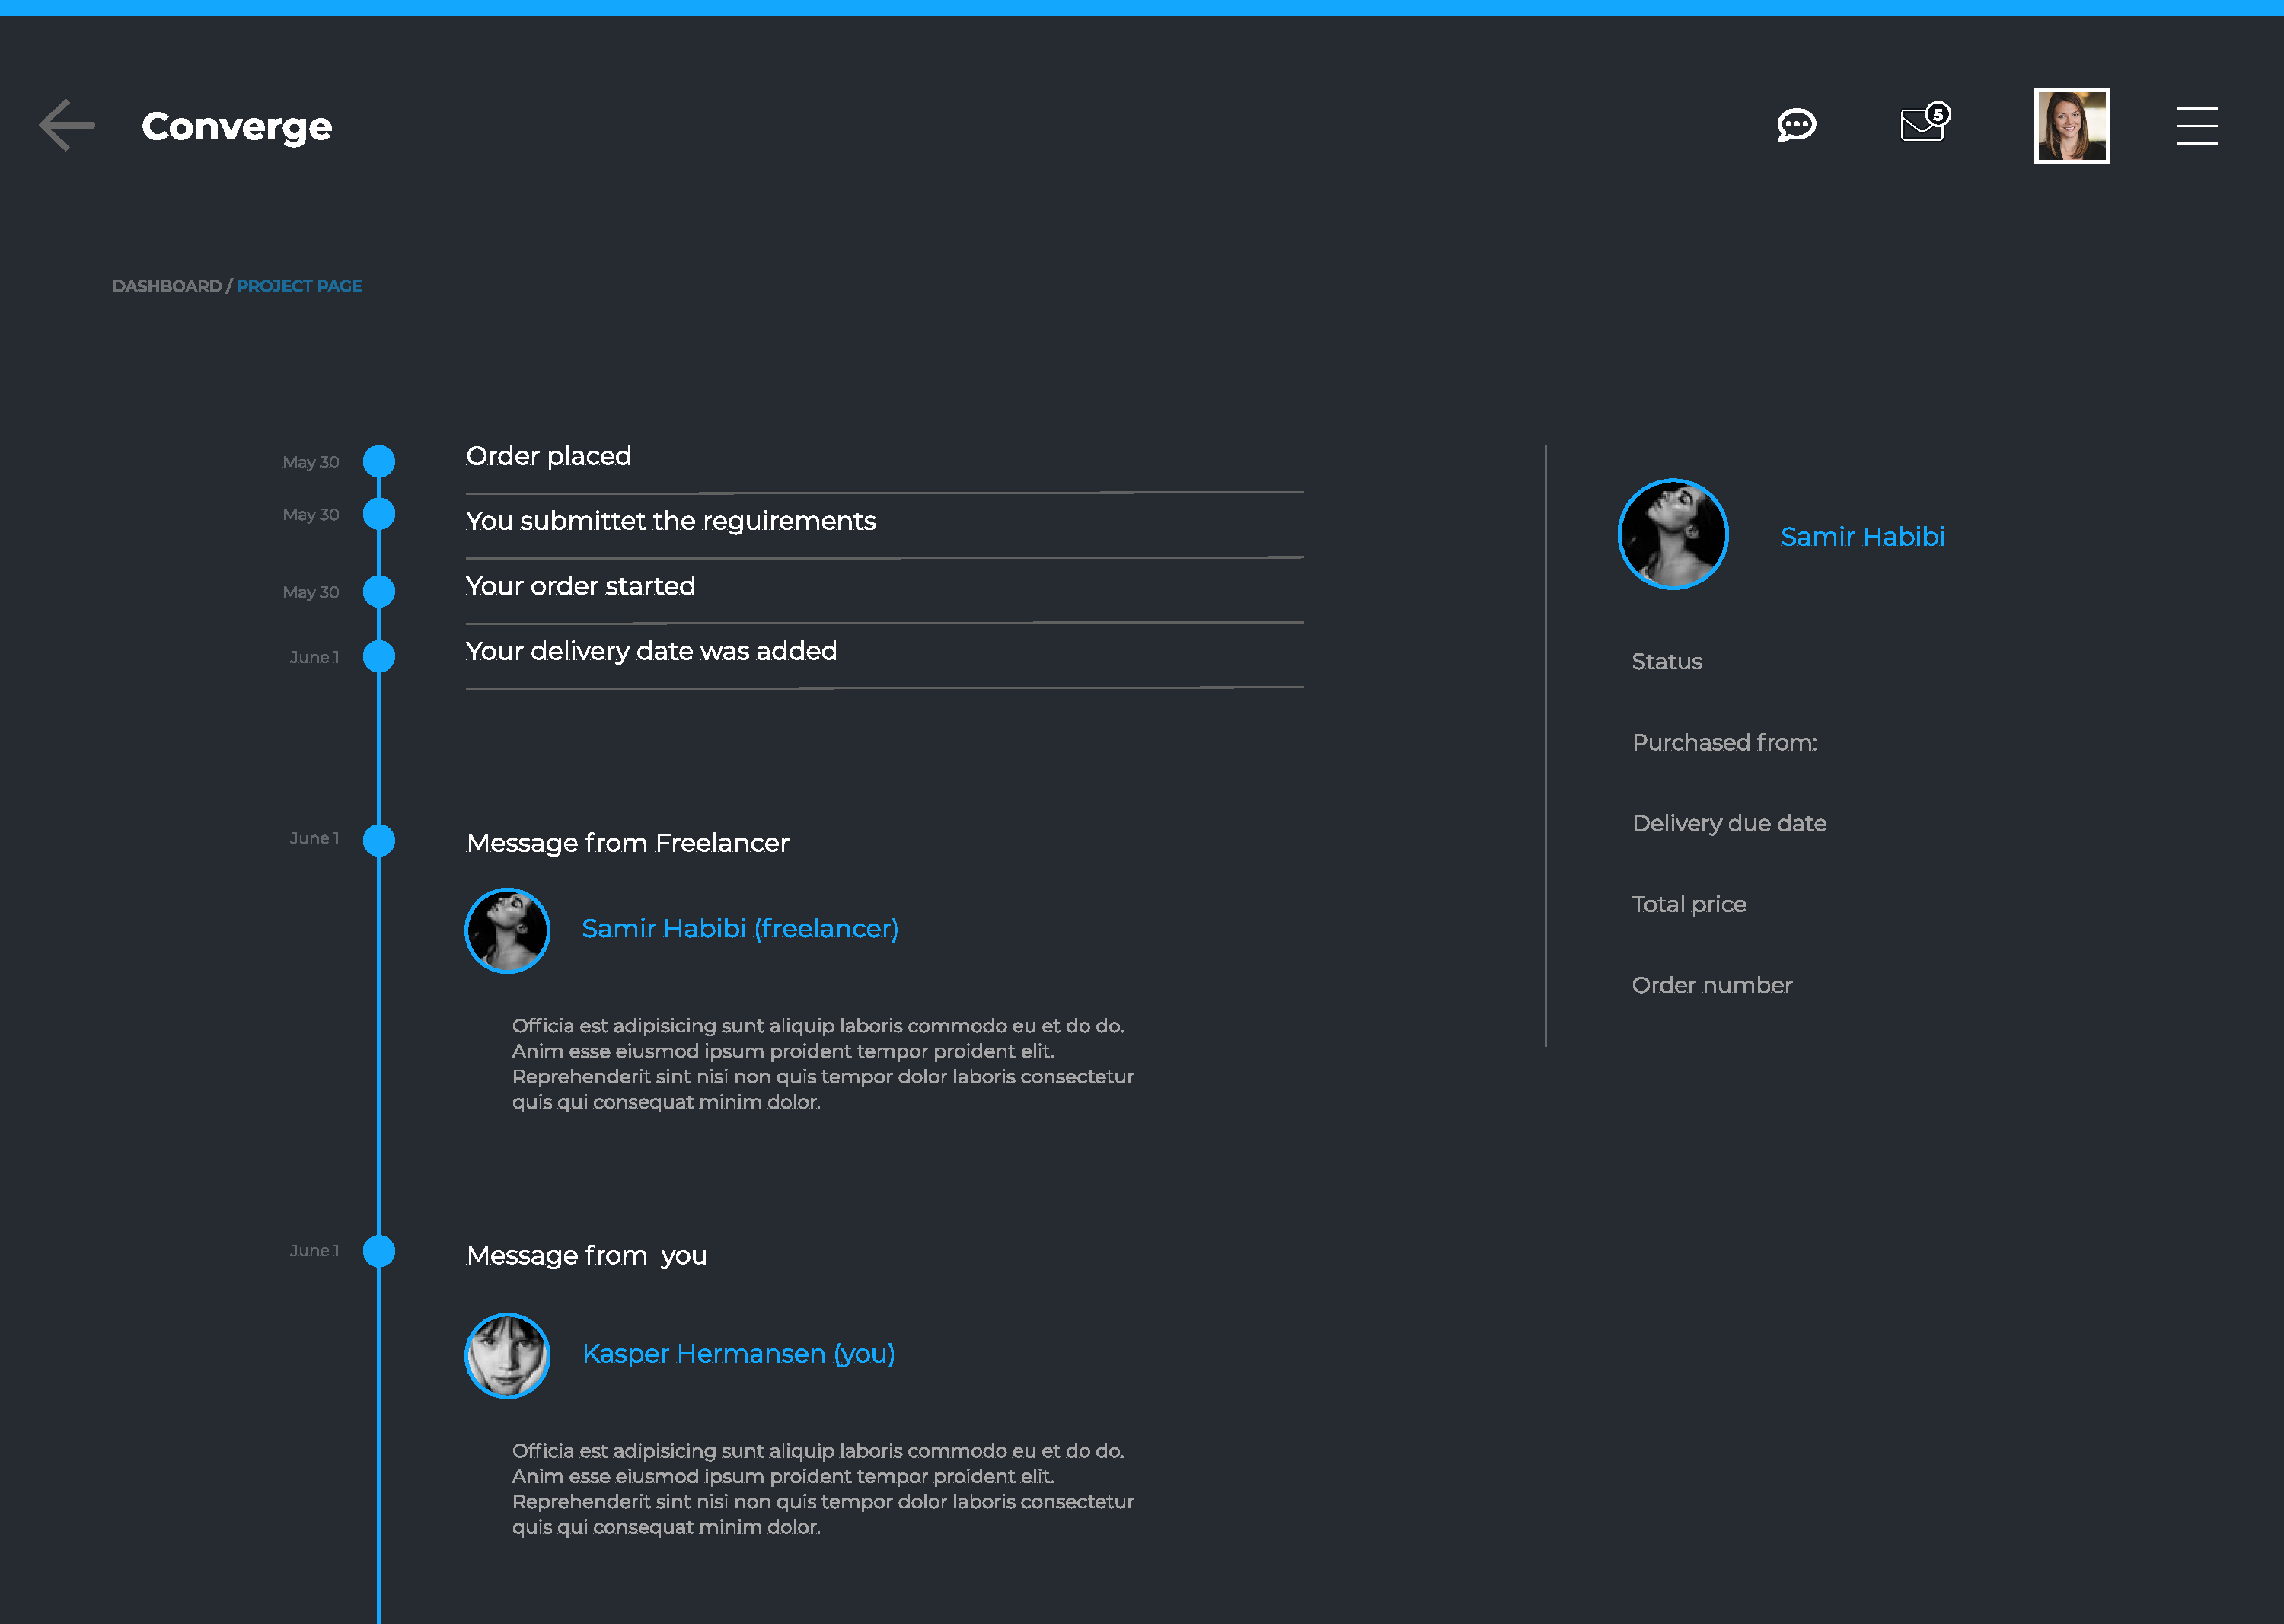
\includegraphics[width=0.6\textwidth]{system-interface-pic/Product.pdf}
\caption{Viser byde siden}
\label{fig:figure2}
\end{figure}

Figur 1.15 viser en tids linje over projektets status, det vil sige her vil brugeren have muglighed for at se hvor langt projektet er, prisen og hvornår projektet blev færdig og afleveret. 